\chapter{Standard Model and Supersymmetry}
\label{chap:SMSUSY}

In this chapter we present first of all, in section \ref{sec:SM}, an overview of the Standard Model (SM), the theory used to describe elementary particles; in section \ref{SMlimits} we move to its main limits and in section \ref{sec:SUSY} we describe one of the most promising extension of the SM, Supersymmetry (SUSY), which is the theoretical framework in which the analysis presented in this thesis is set; current limits on the existence of SUSY particles will be presented. In this chapter and also in the rest of this thesis Natural units will be used, which means that the speed of light, $c$, and the Plank constant, $\hslash$, are normalized to unity and we thus use energy units to describe masses.

\section{Standard Model}
\label{sec:SM}

The Standard Model (SM) is the theory that nowadays best describes elementary particles (or at least the particles that at our present level of understanding we believe to be elementary) and the forces that act between them except from gravity. It has been formulated in the second half of the 20th century \cite{oerter:sm}, and in the last decades it has been tested to a high level of accuracy by many experiments. The predictions of this theory have led to the discovery of many particles and phenomena, like the top quark (discovered in 1995 by the $CDF$ and $D0$ collaborations \cite{cdf:top}, \cite{D0:top}), the tau neutrino (whose observation was announced in 2000 by the DONUT Collaboration \cite{kodama:taunu}), and last but not the least the Higgs boson, recently discovered by the ATLAS and CMS Collaborations at the Large Hadron Collider \cite{atlas:higgs}, \cite{cms:higgs}. 

In this section we will illustrate how particles and their interactions are described in the context of the SM, and how fields originally massless acquire mass through the interaction with the Higgs field.

%%%%%%%%%%%%%%%%%%%%%%%%%%%%%%%%%%%%%%%%%%

\subsection{Fundamental Particles and their Interactions}
\label{smint}
The SM is a gauge quantum field theory based on the group $SU(3) \times SU(2) \times U(1)$, which means that particles are described as excitations of quantum fields \cite{peskin:qft}.

The particles described by the SM and their mass, charge and spin properties are shown in Figure \ref{fig:SMpart}. The SM describes all fundamental forces in nature except from gravity; the interactions described by the SM and the properties of the corresponding gauge bosons are listed in table \ref{tab:sm_interazioni}, and will be further described in the next paragraphs. 
\begin{figure}
\begin{center}
%\includegraphics[width=0.6\textwidth]{./fig/particles.pdf}
\end{center}
\caption{Particles of the Standard Model and their mass, charge and spin properties}
\label{fig:SMpart}
\end{figure}

\begin{table}[h]
\centering
\begin{tabular}{llccc}
\hline
\multirow{2}*{Interaction} & \multirow{2}*{Carrier} & \multirow{2}*{$\frac{Q}{e}$} & \multirow{2}*{Mass [GeV]} & \multirow{2}*{\textbf{$\alpha$}} \\
 & & & &  \\
\hline
\hline
Strong & Gluons (g)  & 0 & 0 & 10 \\
\hline
Electromagnetic & Photon ($\gamma$) & 0 & 0  & $10^{-2}$ \\
\hline
\multirow{2}*{Weak} & $W^{+}$, $W^{-}$    &  +1, -1 &  	$80.385$ $\pm0.015$ GeV   & \multirow{2}*{$10^{-6}$}\\
 & $Z^{0}$  & 0 &  	$91.1876$ $\pm0.0021$ GeV &  \\
\hline
\end{tabular}
\caption[Interaction in the Standard Model]{Interaction in the Standard Model. Here the different force carriers are listed, with their electric charges and masses \cite{pdg:rev}; $\alpha$ is the coupling constant of the different interactions.}
\label{tab:sm_interazioni}
\end{table}

\subsubsection{Fermions}

Matter fields have spin $\frac{1}{2}$, and are called fermions, since they obey Fermi-Dirac statistic and satisfy Pauli exclusion principle: two identical fermions cannot occupy the same quantum state simultaneously. Elementary fermions are further divided in two categories, based on the force they experience. Leptons are fermions that experience only the electroweak force, while quarks are fermions that are subject to both electroweak and strong force. Both leptons and quarks come into three generations of increasing mass. Leptons are observed as free particles, while quarks bind to form composite particles called hadrons, due to a particular property of the strong force that is called confinement. Hadrons are further classified into barions, which have spin $\frac{1}{2}$ and are built of three quarks, and mesons, which have integer spin and are built of 2 quarks. 

In quantum field theory, fermions are described through Dirac spinors, which are fields with four components, that incorporate both particle and antiparticle states. The kinematic of a fermionic field obeys the free Dirac lagrangian:
\beq
 \mathcal{L}_{free} = \bar{\psi} \left( i \gamma^{\mu} \partial_{\mu} - m \right) \psi
 \label{eq:ldirac}
\eeq

Where m is the mass of the fermion, $\gamma^{\mu}$ are the Dirac matrices, that obey anticommutation rules: $\left\lbrace \gamma^{\mu}, \gamma^{\nu}  \right\rbrace = 2 g^{\mu \nu} $, and $\partial_{\mu} $ is the four-vector derivative: $\partial_\mu = ({\partial / \partial t},\, \vec{\nabla})$. Using chirality operators, defined as:
\beq
P_L = (1 - \gamma_5)/2, \qquad\qquad
P_R = (1 + \gamma_5)/2
\eeq

one can project the left or right component of the field:

\beq
\psi_L = \frac{(1 - \gamma_5)}{2} \psi, \qquad\qquad
\psi_R = \frac{(1 + \gamma_5)}{2} \psi
\eeq

In the previous equations, $\gamma_5$ is defined as $\gamma_5 = i \gamma^0 \gamma^1 \gamma^2 \gamma^3 $, and it anticommutes with Dirac matrices:  $\left\lbrace \gamma^{\mu}, \gamma_{5}  \right\rbrace = 0$.

Using these relations one can show that, in the free Dirac lagrangian, the derivative keeps left and right terms separated, while the mass term couples them.



%Beside elementary fermions, described by the SM, there are also composite fermions, such as protons and neutrons, which are built of quarks.

\subsubsection{Bosons}

The SM also describes particles with integer spin, called bosons since they obey Bose-Einstein statistic. The force carriers are spin-1 particles, called gauge bosons. Beside gauge mediators, there is another boson predicted by the SM, the Higgs boson, which has spin 0; the other elementary particles acquire mass trough the interaction with the Higgs boson field as described in section \ref{sec:H}.

In quantum field theory, spin-0 fields obey the kinematics that derives from the free Klein-Gordon lagrangian, which if the field is real is:

\beq
\mathcal{L}_{free} = \frac{1}{2} \partial^\mu \phi \partial_\mu \phi + \frac{1}{2} m^2 \phi ^2 ,
\eeq
 
while for a complex scalar field is:
\beq
\mathcal{L}_{free} =  \partial^\mu \phi \partial_\mu \phi^* +  m^2 \phi \phi^* .
\eeq

On the other hand, a vector field $A^\mu$ with spin 1 obeys the Proca lagrangian if it has mass different from zero
\beq
\mathcal{L}_{free} =  - \frac{1}{4} F^{\mu \nu}F_{\mu \nu}+  \frac{1}{2} m^2 A^\mu A_\mu ,
\label{eq:lproca}
\eeq

and the Maxwell lagrangian if it has null mass

\beq
\mathcal{L}_{free} =  - \frac{1}{4} F^{\mu \nu}F_{\mu \nu} ,
\label{eq:lmax}
\eeq

where we have defined $F^{\mu \nu} = \partial^\mu A_\nu - \partial^\nu A_\mu$

\subsubsection{Gauge Symmetries}

The SM is a gauge theory, which means that interaction terms in the lagrangian are obtained by imposing that a theory which is invariant under a certain transformation retains its invariance also when the transformation becomes local (depends on the space-time coordinates). By invariance of a theory we mean that the lagrangian of the theory (or the action, which is the four-dimensional integral of the lagrangian) is unchanged after a certain transformation of the fields. The simplest example of gauge theory is Quantum Electrodynamics (QED), which will be later on incorporated in the theory of Electroweak Interactions. 

Let's consider Dirac free lagrangian in eq. \ref{eq:ldirac}. It is clearly invariant under the U(1) transformation $\psi \rightarrow e^{i \alpha} \psi$. If we move from a global to a local transformation ($\alpha \rightarrow \alpha (x) $), the theory keeps its invariance if we introduce:
\begin{itemize}
\item A vector field $A^\mu$, which transforms as $A^\mu \rightarrow A^\mu - \partial^\mu \alpha (x)$
\item A Maxwell lagrangian for the vector field like in eq. \ref{eq:lmax}
\item The covariant derivative $D^\mu = \partial^\mu + ieA^\mu$, that substitutes the regular derivative
\end{itemize}
By doing this the lagrangian of the theory becomes:
\beq
\mathcal{L} = \mathcal{L}^{Dirac} + \mathcal{L}^{Maxwell} + \mathcal{L}^{int} \quad \quad \quad \mathcal{L}^{int} = -e \bar{\psi} \gamma^{\mu} \psi A^\mu 
\label{eq:lqed}
\eeq

The term $\mathcal{L}^{int}$ in eq. \ref{eq:lqed} states the form of the allowed interactions between the fermionic field $\psi$ and $A^\mu$, the field of the photon. The only vertex allowed is the one with two fermion fields and one photon field. We can note that using the Proca lagrangian in eq. \ref{eq:lproca} instead of the massless version in eq. \ref{eq:lmax} would introduce a term $\frac{1}{2} m^2 A^\mu A_\mu$, which would not be invariant under gauge transformations, thus spoiling the gauge invariance of the theory.

In a more general gauge theory, the gauge transformation can be described as:
\beq
\psi \rightarrow e^{ig\theta_k \tau_k} \psi  
\eeq

Where $\theta_k = \theta_k(x)$ are space-time dependent functions and $\tau_k$ are the generators of the group and obey commutation relations: 
\beq
\left[ \tau_i, \tau_j \right] = i \epsilon_{ijk} \tau^k 
\eeq
In an Abelian gauge theory, like QED, this commutators are always zero. In a more general theory this is no longer true.

In this case we have to introduce
\begin{itemize}
\item A number of massless gauge fields $W^\mu_k$ equal to the number of generators of the group, that transform as $W^\mu_k \rightarrow W^\mu_k - \partial^\mu \theta_k - g \epsilon_{klm} \theta^m W^\mu_m $
\item A generalization of the covariant derivative of QED, $D^\mu = \partial^\mu + ig\tau^kW^\mu_k$
\item A free lagrangian for the vector fields with $F^{\mu \nu}_k = \partial_\mu W_k^\nu - \partial_\nu W_k^\mu - g \epsilon^k_lm W^\mu_l W^\nu_m$
\end{itemize}
In the last bullet, the tensor $F^{\mu,\nu}$ has a second order term due to the non-Abelian nature of the theory.

The SM is a gauge theory invariant under $SU(3)_C \times SU(2)_L \times U(1)_Y$, where $SU(3)_C$ is the color symmetry of strong interactions and $SU(2)_L \times U(1)_Y$ is the symmetry whose breaking brings to the electroweak interactions. These interactions are described in the next two sections.

\subsubsection{Electroweak Interaction}
The unified theory of electroweak interactions was first proposed by Glashow, Weinberg and Salam in the 1970's. It's a gauge theory based on the group $SU(2)_L \times U(1)_Y$, whose symmetry breaks at an energy scale of about 100 GeV, giving rise to the two interactions that we see at low energy: the electromagnetic interaction and the weak interaction, which can be further classified into weak charged currents (one with a positive and one with a negative charged mediator) and weak neutral currents. These four interactions require four different mediators, therefore the symmetry group of the electroweak theory must have four generators, which is true for the group $SU(2)_L \times U(1)_Y$. The gauge transformation is:
\beq
\psi \rightarrow e^{i \frac{g' \alpha_0}{2}Y} e^{ig \sum_k \alpha_k T^k} \psi ,
\label{eq:wint}
\eeq
where we have introduced T, the weak isospin operator (which is the SU(2) generator), and Y, the weak hypercharge operator. These two quantities are related to the electric charge Q through the relation:
\beq
Q = \frac{Y}{2} + T_3
\eeq
where $T_3$ is the third component of the weak isospin.
In eq. \ref{eq:wint} g is the weak isospin coupling strength, g' the weak hypercharge coupling strength. 

By introducing the covariant derivative we obtain:
\beq
\mathcal{L}_{int}^{EW} = -\frac{g'}{2} \left( \bar{\psi} \gamma_\mu Y \psi \right) B^\mu - g \sum_k \left( \bar{\psi} \gamma_\mu T^k \psi  \right) W_k^\mu
\eeq

Left-handed fields are isospin doublets with the same hypercharge, while right-handed fields are isospin singlets and therefore do not couple to the $W_k^\mu$ fields. When acting on an isospin doublet, the SU(2) generators are just $T^m= \frac{\sigma^m}{2}$, where $\sigma^m$ are the Pauli matrices:

\beq
	\sigma^1 = \left( \begin{array}{cc} 0 & 1 \\ 1 & 0 \end{array} \right) \qquad
	\sigma^2 = \left( \begin{array}{cc} 0 & -i \\ i & 0 \end{array} \right) \qquad
	\sigma^3 = \left( \begin{array}{cc} 1 & 0 \\ 0 & -1 \end{array} \right)
	\label{eq:paulimatrices}
\eeq

The gauge bosons $W_k^\mu$ and $B^\mu$ are the weak interaction eigenstates, which are different from the mass eigenstates, that are obtained by rotating $W_k^\mu$ and $B^\mu$ and requiring the photon field $A^\mu$ to have the correct quantum numbers. By doing this we obtain the physical fields, $W_\mu^\pm$, $A_\mu$, $Z_\mu$ as:

\beq
W_\mu^\pm = \frac{W_\mu^1 \mp W_\mu^2}{\sqrt{2}} \\
A_\mu = B_\mu \cos\theta_W + W^3_\mu \sin\theta_W  \\
Z_\mu = W^3_\mu \cos\theta_W - B_\mu \sin\theta_W
\label{eq:wein}
\eeq

The mixing angle is called Weinberg angle and its experimental value is $\sin^2\theta_W = 0.23113 \pm 0.0005 $. The coupling constants of the isospin and hypercharge are related to the electric charge:

\beq
e = \frac{gg'}{\sqrt{g^2 - g'^2}} \\
e = g \sin\theta_W = g' \cos\theta_W
\eeq

\subsubsection{Strong Interaction}
\label{sec:qcd}
The strong force is the force responsible for binding quarks into hadrons. The theory that describes strong interactions is Quantum Chromo-Dynamics (QCD), and the symmetry group of QCD is SU(3), which means that the transformation of the fields is:
\beq
\psi \rightarrow e^{i \alpha_c^a(x) t^a} \psi
\eeq

Unlike $SU(2)_L \times U(1)_Y$, which is a broken symmetry, $SU(3)_C$ is believed to be an exact symmetry of Nature, therefore the corresponding 8 gauge bosons (called gluons) are massless. Since the group is non-Abelian, the gluons carry color charge and interact not only with quarks but also among themselves. 
The renormalization of a gauge theory implies the definition of running coupling constants, which means that the coupling associated to the vertex of a certain theory is not fixed, but depends on the energy of the process. This is true for both QCD and QED, with the difference that while in QED the coupling constant increases with energy, in QCD it decreases, as shown in eq. \ref{eq:alfaQCD}:

\beq
\alpha(Q^2)=\frac{1}{b\log{\frac{Q^2}{\Lambda_{QCD}^2}}} \quad \quad b = \frac{11N_C-2n_f}{12\pi}
\label{eq:alfaQCD}
\eeq

$N_C$ is the number of colors and $n_f$ is the number of flavor of quarks.  $\Lambda_{QCD}$ represents the energy scale at which the perturbative QCD coupling diverges, and it's known to be around 250 MeV. In QCD $N_C=3$, which means that for $n_f<16$ the coupling constant of QCD shows a decreasing behaviour as the energy increases. This has some important consequences, that define the peculiarities of QCD:

\begin{itemize}
\item Perturbative QCD is valid only at high energies, as long as $\alpha(Q^2) << 1$
\item $\alpha(Q^2) \rightarrow 0$ as $Q^2 \rightarrow \infty $: when the momentum transferred in the interaction is big (which means at small distances), the coupling tends to zero. This behaviour is know as asymptotic freedom.
\item When the momentum transferred is small (large distances) the coupling is really strong, therefore it is not possible to extract quarks from hadrons. This is known as confinement. 
\item When we attempt to extract a quark from a hadron, it is more energetically favoured to create a new quark-antiquark pair. This is known as hadronization and is the reason of the formation of jets of hadrons.
\end{itemize}

%\subsubsection{Flavor Physics and CKM Matrix}


%%%%%%%%%%%%%%%%%%%%%%%%%%%%%%%%%%%%%%%%%%


\subsection{Higgs Physics}
\label{sec:H}

The Higgs boson was the last missing piece of the SM, and its observation in July 2012 is considered one of the milestones of experimental physics. In this section we will first describe how the Higgs mechanism, through spontaneous symmetry breaking, gives masses to elementary particles; then we will briefly present its discovery.

\subsubsection{Higgs Mechanism}

Among the gauge mediators of QED and weak interactions, only the photon is massless. The $W^\pm$ and the Z fields are massive. As we have discussed in section \ref{smint}, a mass term for the gauge bosons in the lagrangian would spoil the gauge invariance of the theory, and thus its renormalizability. For what concerns the fermions, a mass term would couple left-handed and right-handed fields: 

\beq
-m \bar \psi \psi = -m \bar \psi P_L^2 \psi - m \bar \psi P_R^2 \psi
	= -m \bar \psi_R \psi_L - m \bar \psi_L \psi_R
\eeq

We can overcome this problem by introducing a complex scalar field $\Phi$ with non vanishing vacuum expectation value (VEV). The lagrangian for this field is:

\beq
	\mathcal{L}_{\Phi} = ( \mathcal{D}_{\mu} \Phi)^{\dagger} (\mathcal{D}^{\mu} \Phi) - V(\Phi)  \quad \quad V(\Phi) = - \mu^2 \Phi^{\dagger} \Phi + \lambda (\Phi^{\dagger} \Phi)^2
	\label{eq:hpot}
\eeq

In the last equation $\mathcal{D}^{\mu}$ is the covariant derivative:

\beq
\mathcal{D}^{\mu} = \partial^{\mu} + i \frac{g'}{2} B^\mu Y + ig W^\mu_k T^k
\eeq

In the minimal model $\Phi$ is a weak isospin doublet with hypercharge Y=1 and isospin $T=\frac{1}{2}$, whose first component has electric charge Q=+1 and the second one is electrically neutral:

\beq
	\Phi = \left( \begin{array}{c} \phi^+  \\ \phi^0 \end{array} \right)
	= \frac{1}{\sqrt{2}} \left( \begin{array}{c} \phi_1 + i \phi_2 \\ \phi_3 + i \phi_4 \end{array} \right)
\eeq

In equation \ref{eq:hpot}, $\mu^2$ and $\lambda$ are real parameters, defining respectively the strength of the self-interaction of the field ant his mass term. Depending on the sign of these parameters we have different cases:

\begin{itemize}
\item If $\lambda$ is negative the potential V is unbounded from above, so it is not possible to have a stable vacuum state.
\item If $\lambda$ and $-\mu^2$ are both positive, V has a minimum at  $|\Phi| \equiv \sqrt{\Phi^{\dagger} \Phi} = 0$. Since in this case a gauge transformation acting on the vacuum would not change the vacuum, there would be no symmetry breaking.
\item If $\lambda$ is positive and $-\mu^2$ is negative, the minimum of the potential is displaced from zero, as shown in Figure \ref{fig:hpot}.
\end{itemize}

\begin{figure}
\begin{center}
%\includegraphics[width=0.7\textwidth]{fig/higgs_pot.jpg} 
\end{center}
\caption{Potential energy of the Higgs field. On the left panel we see the case where $\lambda$ and $-\mu^2$ are both positive; on the right panel there is the case in which $\lambda >0$ and $-\mu^2 < 0$, and the electroweak symmetry is broken.}
\label{fig:hpot}
\end{figure}

We thus require $\lambda > 0$ and $-\mu^2 < 0$. In this case we actually have a continuum of minima on the circumference of radius:
\beq
\sqrt{\Phi^{\dagger} \Phi} = \sqrt{ \frac{\mu^2}{2 \lambda} } = v
\eeq
The choice of one of these minima selects a vacuum state that is not invariant under a gauge transformation and the symmetry $SU(2)_L \times U(1)_Y$ is spontaneously broken. The $U(1)_Q$ symmetry should not be broken by the choice of the vacuum state. This means that we want $Q \Phi_0 = 0$, where $\Phi_0$ is the selected vacuum state, and this is achieved by setting $< \phi_1 > = 0$, $< \phi_2 > = 0$, $< \phi_4 > = 0$, $< \phi_3 > = v$, as shown in eq. \ref{eq:Qvacuum}

\beq
Q \Phi_0 = \left( \frac{Y}{2} + T_3 \right) \Phi_0 = \frac{1}{2} \left( 1 + \sigma_3 \right) \Phi_0 =  \left( \begin{array}{cc} 1 & 0 \\ 0 & 0 \end{array} \right) \left( \begin{array}{c} 0 \\ v \end{array} \right) = 0
\label{eq:Qvacuum}
\eeq

We can now expand $\Phi$ around its vacuum state:

\beq
	\Phi = \frac{1}{\sqrt{2}} \left( \begin{array}{c} 0 \\ v + \phi \end{array} \right)
\label{eq:hvphi}
\eeq

Here $\phi$ represents the physical field, since it is the displacement from the vacuum. By inserting this expansion in eq. \ref{eq:hpot} and substituting the electroweak gauge fields $W_k^\mu$, $B^\mu$ with the physical fields (with the rotation in eq. \ref{eq:wein}), one obtains the mass terms for the gauge fields $W^\pm$ and $Z$, the mass term for the Higgs field, the strength of the interaction of these fields with the Higgs and its self-interaction.
For what concerns the mass terms:
\beq
M_W^2 = \frac{g^2 v^2}{4}  \\
M_Z^2 = \frac{(g^2 + g^{\prime 2}) v^2}{4}
\eeq
while the field $A^\mu$ does not couple to the Higgs filed, therefore it does not acquire mass. The couplings of the other gauge fields with the Higgs boson are listed in Figure \ref{fig:hww} and \ref{fig:hzz}. We note that the couplings are proportional to the square of the mass of the gauge bosons.

\begin{figure}
\begin{center}
%\includegraphics[width=0.4\textwidth]{fig/2a.pdf} 
%\includegraphics[width=0.4\textwidth]{fig/2b.pdf}
\end{center}
\caption[eynman rules for the $hWW$ and $hhWW$ vertices]{Feynman rules for the $hWW$ and $hhWW$ vertices \cite{arxiv:higgs}.}
\label{fig:hww}
\end{figure}

\begin{figure}
\begin{center}
%\includegraphics[width=0.4\textwidth]{fig/3a.pdf} 
%\includegraphics[width=0.4\textwidth]{fig/3b.pdf}
\end{center}
\caption[Feynman rules for the $hZZ$ and $hhZZ$ vertices]{Feynman rules for the $hZZ$ and $hhZZ$ vertices \cite{martin:primer}.}
\label{fig:hzz}
\end{figure}

Introducing eq. \ref{eq:hvphi} in eq. \ref{eq:hpot} we find that the potential V can be expressed as:
\beq
V(\Phi) = \frac{\lambda}{4} \left( v + \phi \right)^4 - \frac{\mu^2}{2} \left( v + \phi \right)^2 = const + 2 \mu^2\phi^2 + 2 \sqrt{2}\frac{\mu}{\sqrt{\lambda}} \phi^3 + \lambda \phi^4
\eeq
Hence yielding a tree level Higgs mass of:
\beq
M_H = \sqrt{2} \mu
\eeq
And the self-couplings reported in Figure\ref{fig:hhh}.
\begin{figure}
\begin{center}
%\includegraphics[width=0.4\textwidth]{fig/5a.pdf} 
%\includegraphics[width=0.4\textwidth]{fig/5b.pdf}
\end{center}
\caption[Feynman rules for the $hhh$ and $hhhh$ vertices]{Feynman rules for the $hhh$ and $hhhh$ vertices \cite{martin:primer}.}
\label{fig:hhh}
\end{figure}

The mass terms for fermions are obtained introducing by hand a Yukawa coupling term between the fermionic fields and the Higgs field. Because of this, the coupling constant is a free parameter assumed to be proportional to the mass of the fermion, which is not constrained by the parameters of the theory, in contrast with the mass of the gauge bosons.
To give masses to up-type fermions through the mechanism of the spontaneous symmetry breaking, we need to introduce the complex conjugate of the Higgs doublet, given by:

\beq
 \Phi_C = i \sigma^2 \Phi^* 
	= i \left( \begin{array}{cc} 0 & -i \\ i & 0 \end{array} \right) 
	\left( \begin{array}{c} \phi^- \\ \phi^{0*} \end{array} \right)
	= \left( \begin{array}{c} \phi^{0*} \\ - \phi^- \end{array} \right)
\eeq

This way we can write the Yukawa term in the lagrangian as:
%\beq
%\mathcal{L}_{Yukawa} &=& - \left[  g_d \left( \bar{u}_L \,\, \bar{d}_L  \right) \Phi d_R +  g_u \left( \bar{u}_L \,\, \bar{d}_L  \right) \Phi_C u_R \right] + h.c. \\
%&=& - \frac{1}{\sqrt{2}} \left[  g_d \left( v + \phi \right) \bar{d}_L d_R + h.c. + g_u \left( v + \phi \right) \bar{u}_L d_u + h.c. \right] \nonumber
%\eeq

We now recognize the fermion mass terms:
\beq
M_{u,d} =  \frac{1}{\sqrt{2}} v g_{u,d}
\eeq

And the couplings to the Higgs boson, reported in Figure\ref{fig:hee}.

\begin{figure}
\begin{center}
%\includegraphics[width=0.4\textwidth]{fig/4.pdf} 
\end{center}
\caption[Feynman rules for the $hee$ vertex]{Feynman rules for the $hee$ vertex}
\label{fig:hee}
\end{figure}


\subsubsection{Discovery and Measurements of the Higgs Boson}

On July 4th 2012 the ATLAS and CMS experiments announced they had independently discovered a previously unknown boson, with properties compatible with those expected for the Higgs boson. The discovery was made using the data collected in 2011 ($\approx 5 fb^{-1}$ at \cmsette) and the first data of 2012 ($\approx 5 fb^{-1}$ at \cmotto), combining the results of two of the decay channels of the Higgs, $H \rightarrow \gamma \gamma $ and $H \rightarrow Z Z^* \rightarrow llll $, which are the channels where the invariant mass of the parent particle can be most easily reconstructed. 

Since 2012, measurements have been updated with the full \cmotto dataset ($\approx 20 fb^{-1}$, for a total of $\approx 25 fb^{-1}$). The invariant distributions of the decay products for these two channels is shown in Figure\ref{fig:hmass}, while in Figure \ref{fig:hsig} we see the Fit of $m_H$ and likelihood contours as a functions of the normalized signal yield $S= \frac{\sigma}{\sigma_{SM,mH = 125.36 \; GeV}}$ and $m_H$ for the individual $H \rightarrow \gamma \gamma $ and $H \rightarrow Z Z^* \rightarrow llll $ channels and their combination \cite{atlas:hmass}.

\begin{figure}[h]
\centering
%\includegraphics[width=.45\columnwidth]{./fig/hgammagamma.pdf}
%\includegraphics[width=.45\columnwidth]{./fig/h4l.pdf}
\caption[Invariant mass of the candidate Higgs boson in the $\gamma \gamma $ and 4-lepton channels]{(a) Invariant mass distribution in the $H \rightarrow \gamma \gamma $ analysis for data (7 TeV and 8 TeV samples combined). (b) Distribution of the four-lepton invariant mass for the selected candidates in the $m_{4l}$ range 80-170 GeV for the combined 7 TeV and 8 TeV data samples. Superimposed are the expected distributions of a SM Higgs boson signal for $m_H=124.5$ GeV normalized to the measured signal strength, as well as the expected $ZZ^*$ and reducible backgrounds \cite{atlas:hmass}. }
\label{fig:hmass}
\end{figure}

%\begin{figure}[h]
%\centering
%{\includegraphics[width=.45\columnwidth]{./fig/mh.pdf}} \quad
%{\includegraphics[width=.45\columnwidth]{./fig/signalstrenghth.pdf}} 
%\caption[Fit of $m_H$ and likelihood contours]{Results for the individual $H \rightarrow \gamma \gamma $ and $H \rightarrow Z Z^* \rightarrow llll $ channels and their combination. (a) Fit of $m_H$. (b) Likelihood contours as a functions of the normalized signal yield $S= \frac{\sigma}{\sigma_{SM,mH = 125.36 \; GeV}}$ and $m_H$  \cite{atlas:hmass}.}
%\label{fig:hsig}
%\end{figure}

The updated mass measurement is now:

\beq
\nonumber
m_H^{ATLAS} = 125.36 \pm 0.37(stat)\pm 0.18 (syst) \,\, GeV \\ \nonumber
m_H^{ATLAS} = 125.03 ^{+0.26}_{-0.27}(stat)^{+0.13}_{-0.15}  (syst) \,\, GeV 
\eeq

The observation of this new resonance now exploits also the channels $\tau \tau$ and $WW^* \rightarrow l \nu l \nu$, and the evidence is more than 7 $\sigma$. To prove that this new resonance is the Higgs boson, other properties beside its mass have to be tested. In particular, this resonance has spin-parity properties compatible with $J^P=0^+$, and $2^+$, $1^\pm$ and $0^-$ are disfavoured at more than 99\% CL.

%\clearpage

%%%%%%%%%%%%%%%%%%%%%%%%%%%%%%%%%%%%%%%%%%

\section{Limits of the Standard Model}
\label{SMlimits}

The SM is well verified at an high level of accuracy, but there are some hints that it might not be the fundamental theory that describes Nature. In this section we will describe some of these characteristics, with particular emphasis on those solved by Supersymmetry.

\subsubsection*{Neutrino Masses}
The SM predicts neutrinos with null mass, while experimental observation of neutrino oscillations proves that neutrinos have mass different from zero.

\subsubsection*{Hierarchy Problem}
In section \ref{sec:H} we obtained the Higgs mass term, but that was only the tree level approximation. The correct calculation of the Higgs mass should include radiative corrections to the Higgs propagator coming from loops of all the other particles coupling to the Higgs boson. In particular, for fermions the coupling with the Higgs is given by a Yukawa term, $-\lambda_f \phi \bar{f} f$. The loop integrals originating from these corrections are divergent, and the regularization of the theory requires a cut-off; since we know that at the Plank scale, $10^{19}$ GeV, the SM is not anymore valid, e reasonable cut-off for the momentum of the particles in the loop is the Plank scale itself; at an higher energy scale, new physics beyond the SM must enter the theory. The contribution to the Higgs mass given by a loop of fermions as the one shown in figure \ref{fig:hcorr}(a) is given by:

\beq
\Delta m_H^2 \>=\>  
-{|\lambda_f|^2\over 8 \pi^2} \Lambda_{cut-off}^2 + \ldots
\label{eq:divhf}
\eeq

where the ellipses are meant to represent the other terms logarithmic in $\Lambda_{cut-off}$. The corrections to the mass are thus of the same order of magnitude of the cut-off scale. To yield a Higgs mass of about 125 GeV, these corrections from radiative terms should cancel out with the bare Higgs mass term. This requires a fine tuning of the parameters, which should be of the order of $\frac{m_H}{\Lambda} \approx 10^{-17}$. 

All the fermions of the SM contribute to the correction to the Higgs propagator. However, since the couplings of fermions to the Higgs boson (and thus their contribution to the radiative corrections to the propagator) are proportional to their masses, the largest correction is given by the loop of the top quark.

A possible solution could be to choose a cut-off scale not too large, but in that case one should have new physics entering the theory at that scale. On the other hand, if we consider a massive scalar particle S, for dimensional arguments its coupling to the Higgs boson should be of the form $ -\lambda_S
|\phi|^2 |S|^2$. In this case the correction to the propagator, shown in figure \ref{fig:hcorr}(b), is given by:
 
\beq
\Delta m_H^2 \>=\> {\lambda_S\over 16 \pi^2}
\left [\Lambda_{cut-off}^2 - 2 m_S^2
\> {\rm ln}(\Lambda_{cut-off}/m_S) + \ldots
\right ].
\label{eq:divhs}
\eeq 
 
We note that in the two equations \ref{eq:divhf} and \ref{eq:divhs}, the corrections to the squared mass have opposite sign. If we imagine to associate to each fermion of the SM two complex scalars such that $\lambda_S = |\lambda_f|^2$, the two contributions would cancel each other. As we will see in the next sections, this is what is postulated by Supersymmetry (SUSY). 

\begin{figure}
\begin{center}
%%\includegraphics[width=0.7\textwidth]{fig/higgs_corr.pdf} 
\end{center}
\caption[Loop corrections to the Higgs boson propagator]{Loop corrections to the Higgs boson propagator, coming from a fermion (a) and a scalar (b)}
\label{fig:hcorr}
\end{figure}

\subsubsection*{Unification of coupling constants}

As we have discussed in section \ref{sec:qcd}, the QCD coupling constant decreases with energy, while the $U(1)_Y$ and $SU(2)_L$ couplings have the opposite behaviour. If the SM were the low energy limit of a simpler gauge theory, with only one coupling constant, the values of the three different coupling constants of the SM should converge at high energy in one single point, as predicted by grand unification theories. The renormalization group equations in the SM are such that there is no energy scale at which this happens. In SUSY theories the particle content is different, and in some models, like the Minimal Supersymmetric Standard Model (MSSM), this unification can take place, as shown in figure \ref{fig:couplings}.

\begin{figure}
\begin{center}
%\includegraphics[width=0.45\textwidth]{fig/unification_couplings.pdf} 
\end{center}
\caption[Evolution of the coupling constants]{Evolution of the inverse of the gauge couplings in the SM (dashed lines) and in the Minimal Supersymmetric Standard Model, one of the SUSY models. In the SUSY scenario the convergence if the couplings to a single value at high energies is better than in the SM.}
\label{fig:couplings}
\end{figure}

\subsubsection*{Dark Matter and Dark Energy}
The SM describes only ordinary matter, which is made of fermions and hadrons. From cosmological results, we now that ordinary matter accounts only for the 4\% of the content of the universe. First of all, not all the matter behaves like ordinary matter. The rotational velocity of the galaxies does not decrease with the distance from the center of the galaxies as it should if the content of matter was in a one to one correspondence with the light we see; this implies that there is another kind of matter, that is subject to gravitational force but does not shine. This kind of matter is called dark matter, and accounts for another 22\% of the energy content of the universe. The remaining 76\% it thought to be dark energy, which is responsible for the accelerated expansion of the universe.

Supersymmetric theories that are R-parity conserving (described in section \ref{sec:rpar}), supply a good candidate for dark matter, the Lightest Supersymmetric Partner (LSP). Nowadays there is not a field theory able to propose a good candidate for dark energy.


\subsubsection*{Barionic Asimmetry of the Universe}
In the context of the SM, the CKM matrix with its complex phase offers a source of CP asymmetry. This is however not enough to explain the asymmetry between the content of matter and anti-matter that we observe in our universe.

\subsubsection*{Charge Quantization}
While the quantization of the angular momentum is explained by the non-Abelian nature of the SU(2) group, the symmetry group of QED, U(1), is Abelian, and so it does not require the conserved quantity (the electric charge) to be quantized. 

Also the choice of the hypercharge Y is arbitrary, and it is assigned so that the electron charge and the proton charge, which in principle should be two independent parameters of the SM, have the same absolute value.

\subsubsection*{Gravity}
The SM describes only three of the four fundamental forces (electromagnetic, weak and strong), while gravity is not included in this theory. This is a conceptual problem, but it also limits the validity of the theory to the scale at which gravity effects become comparable to the effects of the other forces acting between elementary particles; this is known as Plank scale, and it is about $10^{19}$ GeV. 

\subsubsection*{Free Parameters}
The free parameters of the SM are:
\begin{itemize}
\item 9 fermion masses (+ 3 if $m_\nu$ is different from zero)
\item 3 angles and 1 phase for the CKM matrix (+ 3 + 1 if $m_\nu$ is different from zero)
\item 3 coupling constants for U(1), SU(2), SU(3)
\item 1 for the Higgs mass and 1 for the Z mass (the masses of the other gauge bosons can be obtained form these)
\end{itemize}
So we have 18 free parameters, which become 25 if we include neutrino masses. This large number of free parameters is seen as a hint of the SM not being a fundamental theory.


%%%%%%%%%%%%%%%%%%%%%%%%%%%%%%%%%%%%%%%%%%
%%%%%%%%%%%%%%%%%%%%%%%%%%%%%%%%%%%%%%%%%%
%%%%%%%%%%%%%%%%%%%%%%%%%%%%%%%%%%%%%%%%%%

\section{Supersymmetry}
\label{sec:SUSY}

Supersymmetry (SUSY) is one of the most attractive extensions of the SM \cite{martin:primer}. In this section an introduction to SUSY will be given. Then we will take a look at the simplest SUSY model, Wess-Zumino model, and techniques used to include interactions in it.

%%%%%%%%%%%%%%%%%%%%%%%%%%%%%%%%%%%%%%%%%%

\subsection{Introduction}
\label{sec:susyintro}

A supersymmetry transformation rotates a bosonic state into a fermionic state and vice-versa. The operator that generates this transformation is Q, the supercharge:

\beq
Q |{\rm Boson}\rangle = |{\rm Fermion }\rangle \qquad\qquad
Q |{\rm Fermion}\rangle = |{\rm Boson }\rangle .
\eeq

Since Q interchanges bosonic and fermionic states, it must carry a fermionic index. $Q^\dagger$, the hermitian conjugate of Q, is also a symmetry generator. The spinorial nature of the  supercharge operator seems to be in contrast with Coleman-Mandula theorem, that states that ``space-time and internal symmetries cannot be combined in any but a trivial way'' \cite{coleman:mandula}; this implies that the generators of the internal transformations should be scalar. 
This problem was solved by the Haag-Lopuszanski-Sohnius extension of the theorem, that allows such fermionic generators and puts restrictions on the algebra of commutation and anticommutation relations they must satisfy, called supersymmetry algebra:

%\beq
%&&\{ Q, Q^\dagger \} = P^\mu , \label{eq:susyalgone}
%\\
%&&\{ Q,Q \} = \{ Q^\dagger , Q^\dagger \} = 0 , \label{eq:susyalgtwo}
%\\
%&&[ P^\mu , Q  ] = [P^\mu, Q^\dagger ] = 0 ,\label{eq:susyalgthree}
%\eeq

where $P^\mu$ is the four-momentum operator, the generator of space-time translations. Equation \ref{eq:susyalgone} states that by applying a combination of the supercharge operator and its hermitian conjugate one can obtain a translation in space-time.


The irreducible representations of the supersymmetry algebra (the particles predicted by the theory) are classified into supermultiplets, that include SM particles and the particles that SUSY associates them, called superpartners. Equation \ref{eq:susyalgthree} implies that $[ (P^\mu)^2 , Q  ]=0$, so all particles inside the same supermultiplet should have the same mass. It can also be sown that, within a single supermultiplet, the number of fermionic degrees of freedom has to be equal to the number of bosonic degrees of freedom. This gives us a guideline to construct and classify supermultiplets:

\begin{description}

\item[Chiral supermultiplet] If we consider a Weyl fermion, it has two helicity states and so two degrees of freedom; it then needs to be matched with two real scalar fields which, since a Weyl fermion is a complex object, are naturally merged into a single complex field. The superpartner of a fermion is called sfermion (it stands for scalar-fermion), so we have that the superpartner of the electron is called selectron, the superpartner of the top quark is called stop and so on. From the graphical point of view, superpartners are indicated with the same letter identifying the SM particles, but with a $\texttildelow$ on top of it. For example the superpartner of the $e_L$ is the $\tilde{e}_L$. We notice that, in the case of sfermions, the L,R subscript looses its meaning of helicity (sfermions are scalars) and it only refers to helicity of the SM partner. The Higgs sector of SUSY gives rise to two chiral supermultiplets as well.

\item[Gauge supermultiplet] Gauge bosons are spin 1 particles and, before symmetry breaking, they are massless. A massless spin 1 particle has 2 bosonic degrees of freedom, which means it has to be associated with a spin $\frac{1}{2}$ Weyl fermion; these fermions have the same name of the SM particles but with a -ino suffix (gauginos). Since gauge bosons belong to the adjoined representation of the gauge group (which is its own conjugate), left-handed and right-handed gauginos must have the same gauge transformation. 

\item[Gravitational supermultiplet] If we want a theory that includes gravity, we have to postulate the existence of a massless spin 2 graviton. Its superpartner, the gravitino, has to be a spin $\frac{3}{2}$ particle.

\end{description}

The chiral multiplets of a minimal supersymmetric extension of the SM, their spin and properties under gauge transformations are reported in table \ref{tab:chiral}, while the gauge multiplets are reported in table \ref{tab:gauge}. We have to notice that these particles do not have to be mass eigenstates, since there can be mixing between the electroweak gauginos and higgsinos, and between the sfermions associated with the left-handed or right-handed component of a SM particle. The only SUSY particles that do not mix are gluinos, since they do not have the correct quantum numbers to mix with other particles.

It is worth noticing that, in table \ref{tab:chiral}, the Higgs sector is more extended than one could think. It seems natural that the Higgs boson, being a spin-0 particle, has to be part of a chiral supermultiplet. But the minimum content of Higgs supermultiplets in SUSY is two. There are different arguments to prove this, one of them being the need to avoid introducing a gauge anomaly in the theory. In order for the gauge anomalies to cancel, we need to have $\sum Tr \left[Y^3  \right]$, where Y is the hypercharge and the sum runs over all the left-handed fermions of the theory; this condition is satisfied in the SM. If we introduce only one Higgs supermultiplet, the superpartner of the Higgs would be a weak isospin doublet with $Y=\frac{1}{2}$ or $Y=-\frac{1}{2}$. In both cases, the new fermion would spoil the cancellation of anomalies. This can be avoided by introducing two Higgs sumpermultiplets, one with $Y=\frac{1}{2}$ and one with $Y=-\frac{1}{2}$.

\renewcommand{\arraystretch}{1.4}
\begin{table}[tb]
\begin{center}
\begin{tabular}{c c c c c}
\hline
\multicolumn{2}{c}{Names} 
& spin 0 & spin 1/2 & $SU(3)_C ,\, SU(2)_L ,\, U(1)_Y$
\\  \hline\hline
squarks, quarks & $Q$ & $({\stilde u}_L\>\>\>{\stilde d}_L )$&
 $(u_L\>\>\>d_L)$ & $(\>{\bf 3},\>{\bf 2}\>,\>{1\over 6})$
\\
($\times 3$ families) & $\sbar u$
&${\stilde u}^*_R$ & $u^\dagger_R$ & 
$(\>{\bf \overline 3},\> {\bf 1},\> -{2\over 3})$
\\ & $\sbar d$ &${\stilde d}^*_R$ & $d^\dagger_R$ & 
$(\>{\bf \overline 3},\> {\bf 1},\> {1\over 3})$
\\  \hline
sleptons, leptons & $L$ &$({\stilde \nu}\>\>{\stilde e}_L )$&
 $(\nu\>\>\>e_L)$ & $(\>{\bf 1},\>{\bf 2}\>,\>-{1\over 2})$
\\
($\times 3$ families) & $\sbar e$
&${\stilde e}^*_R$ & $e^\dagger_R$ & $(\>{\bf 1},\> {\bf 1},\>1)$
\\  \hline
Higgs, higgsinos &$H_u$ &$(H_u^+\>\>\>H_u^0 )$&
$(\stilde H_u^+ \>\>\> \stilde H_u^0)$& 
$(\>{\bf 1},\>{\bf 2}\>,\>+{1\over 2})$
\\ &$H_d$ & $(H_d^0 \>\>\> H_d^-)$ & $(\stilde H_d^0 \>\>\> \stilde H_d^-)$& 
$(\>{\bf 1},\>{\bf 2}\>,\>-{1\over 2})$
\\  \hline
\end{tabular}
\caption{Chiral supermultiplets in the Minimal Supersymmetric Standard Model.
The spin-$0$ fields are complex scalars, and the spin-$1/2$ fields are 
left-handed two-component Weyl fermions.\label{tab:chiral}}
\vspace{-0.6cm}
\end{center}
\end{table}


\renewcommand{\arraystretch}{1.55}
\begin{table}[t]
\begin{center}
\begin{tabular}{c c c c}
\hline
Names & spin 1/2 & spin 1 & $SU(3)_C, \> SU(2)_L,\> U(1)_Y$\\
\hline\hline
gluino, gluon &$ \stilde g$& $g$ & $(\>{\bf 8},\>{\bf 1}\>,\> 0)$
\\
\hline
winos, $W$ bosons & $ \stilde W^\pm\>\>\> \stilde W^0 $&
 $W^\pm\>\>\> W^0$ & $(\>{\bf 1},\>{\bf 3}\>,\> 0)$
\\
\hline
bino, B boson &$\stilde B^0$&
 $B^0$ & $(\>{\bf 1},\>{\bf 1}\>,\> 0)$
\\
\hline
\end{tabular}
\caption{Gauge supermultiplets in
the Minimal Supersymmetric Standard Model.\label{tab:gauge}}
\vspace{-0.45cm}
\end{center}
\end{table}

%%%%%%%%%%%%%%%%%%%%%%%%%%%%%%%%%%%%%%%%%%
%%%%%%%%%%%%%%%%%%%%%%%%%%%%%%%%%%%%%%%%%%

\subsection{Supersymmetric Lagrangians and Super-Multiplets}

In this section we give an overview of the simplest SUSY model and how SUSY-invariant interactions are included into it.

\subsubsection*{Wess-Zumino Model}

We want now to build the simplhiggsest supersymmetric model, called Wess-Zumino model, starting from a theory that contains only a left-handed Weyl spinor $\psi$ and a complex scalar field $\phi$. The free lagrangian for this theory is:

\beq
\mathcal{L}_{WZ} = \partial^\mu \phi^* \partial_\mu \phi + i \psi^\dagger \bar{\sigma}^\mu \partial_\mu \psi
\label{eq:WZL}
\eeq

This is the massless, non interacting Wess-Zumino lagrangian. The corresponding action, which is the four-dimensional integral of the lagrangian, is:

\beq
S_{WZ} = \int d^4x \; \mathcal{L}_{WZ}
\eeq

We now introduce an infinitesimal parameter $\epsilon$ with a fermionic index: 
%$\epsilon \equiv \binom{\epsilon^1}{\epsilon^2}$, 
% chiara: decomment
that does not depend on the space-time coordinates (global symmetry). We define an infinitesimal transformation of both the scalar and the chiral fields:

\beq
\delta \phi = \epsilon^\dagger \psi \qquad ;  \qquad \delta \psi = -i(\sigma^\nu \epsilon)\partial_\nu \phi 
\delta \phi^* = \psi^\dagger \epsilon \qquad  ; \qquad \delta \psi^\dagger = i(\epsilon^\dagger \sigma^\nu )\partial_\nu \phi^*
\eeq

It can be shown that the Wess-Zumino action is invariant under these transformations, that constitute then a symmetry of the system (Supersymmetry). The field $\binom{\phi}{\psi}$  is a supermultiplet.

%%%%%%%%%%%%%%%%%%%%%%%%%%%%%%%%%%%%%%%%%%

\subsubsection*{Chiral Super-Multiplets}

The Wess-Zumino lagrangian as in eq. \ref{eq:WZL} does not provide a particularly interesting model, since it does not include interactions. In order to introduce interactions in the theory, we write the most general potential which is invariant under SUSY transformations and is renormalizable. The lagrangian has the form:

%\beq
% \begin{split}
%  \mathcal{L}_{chiral}^{int} &= -\frac{1}{2} \left( W^{i,j} \psi_i \psi_j + W^*_{i,j} \psi^{ \dagger i}  \psi^{ \dagger j} \right) + W^i W^*_i = \\
%  								& =  -\frac{1}{2} \left( M^{i,j} \psi_i \psi_j + M^*_{i,j} \psi^{ \dagger i}  \psi^{ \dagger j} \right) + M^{ij} M^*_{ik} \phi_j \phi^{* k} + \\
%  								& -\frac{1}{2} \left( y^{ijk} \psi_i \psi_j \phi_k + y^*_{ijk} \psi^{\dagger i} \psi^{\dagger j} \phi^{* k} \right) + \\
%  								& + \frac{1}{2} \left(  M^{ij} y^*_{ikl} \phi_j \phi^{*k} \phi^{*l}      +    M^*_{ij} y^{ikl} \phi_k \phi_l \phi^{*j}    \right) + \\			& +\frac{1}{4} y^{ijk} y^*_{ilm} \phi_j \phi_k \phi^{*l} \phi^{*m} ,
%\end{split}
%\label{eq:lint}
%\eeq

where we have introduced the Superpotential:

\beq
W =
{1\over 2} M^{ij} \phi_i \phi_j + {1\over 6} y^{ijk} \phi_i \phi_j \phi_k,
\label{superpotential}
\eeq

and its derivatives:

\beq
W^i \equiv \frac{\partial W}{\partial \phi_i} = M^{ij} \phi_j + \frac{1}{2} y^{ijk} \phi_j \phi_k 
\\
W^{ij} = {\delta^2 \over \delta\phi_i\delta\phi_j} W = M^{ij} + y^{ijk} \phi_k
\eeq

The Superpotential has to be a holomorfic function of the chiral superfields; this will play an important role in the definition of the Higgs sector of the MSSM. In equ. \ref{eq:lint} we have used the notation:

\beq
\psi_i \psi_j = \psi_i^T \begin{pmatrix}
0 & -1 \\ 1 & 0
\end{pmatrix} \psi_j
\\
\psi^{\dagger i} \psi^{\dagger j} \equiv \left(  \psi^i \psi^j   \right)^*
\eeq

The overall chiral lagrangian becomes:

\beq
 \begin{split}
  \mathcal{L}_{chiral} &=  \partial^\mu \phi^{* i} \partial_\mu \phi_i  M^{ij} M^*_{ik} \phi_j \phi^{* k} +    \; \; \;  massive \, scalars\\
&  + i \psi^{\dagger i} \bar{\sigma}^\mu \partial_\mu \psi_i + -\frac{1}{2} \left( M^{i,j} \psi_i \psi_j + M^*_{i,j} \psi^{ \dagger i}  \psi^{ \dagger j} \right) + \; \; \; massive \; fermions \\
  & -\frac{1}{2} \left( y^{ijk} \psi_i \psi_j \phi_k + y^*_{ijk} \psi^{\dagger i} \psi^{\dagger j} \phi^{* k} \right) +  \; \; \; scalar-fermion-fermion\, int. \\
   	& + \frac{1}{2} \left(  M^{ij} y^*_{ikl} \phi_j \phi^{*k} \phi^{*l}      +    M^*_{ij} y^{ikl} \phi_k \phi_l \phi^{*j}    \right) + \; \; \;  3-scalar \, int. \\ 
   & +\frac{1}{4} y^{ijk} y^*_{ilm} \phi_j \phi_k \phi^{*l} \phi^{*m}\; \; \; 4-scalar\,int. 
\end{split}
\label{eq:lchiral}
\eeq

A dimensional analysis of the quantities in eq. \ref{eq:lchiral} yields, in mass units: $[S]=0, \; [\mathcal{L}]=4, \; [\phi]=1, \;  [\psi]= \frac{3}{2}$. Therefore: $[M^{ij}]=1, \; [W]=3, \; [y^{ijk}]=0$. We notice then that the Superpotential is not a potential in the ordinary sense, since it does not have the dimensions of an energy. It is important to notice that the Superpotential contains only the fields and not their complex conjugates. 

Once we assign all the $M^{ij}$ and the $y^{ijk}$, we have determined all the properties of the theory.




\subsubsection*{Masses of a Chiral Supermultiplet}

We can compute the masses of the scalar and the fermion by looking at the linearized equations of motion. We start form \ref{eq:lchiral}, write the Eulero-Lagrange equations and keep only the terms with a single field (we want to study the free system). For the scalar field:

\beq
\frac{\delta \mathcal{L}}{ \delta \phi^{*k}   } = M^{ij} M^*_{ik} \phi_j        + \mathcal{O}(\geqslant 2) \quad \quad \quad \frac{\delta \mathcal{L}}{ \delta  (\partial_\mu \phi^{*k})   } = \partial^\mu \phi_k 
\eeq

And so:
\beq
\partial_\mu \partial^\mu \phi_k = (\mathcal{M}^2)_k^{\, j} \phi_j + \mathcal{O}(\geqslant 2)
\eeq
Where we have defined  $M^{ij} M^*_{jk} \equiv (\mathcal{M}^2)^i_{\, k}$. For the fermions:

\beq
\frac{\delta \mathcal{L}}{ \delta  \psi^{\dagger k}  } = i \bar{\sigma}^\mu \partial_\mu \psi_K - M^*_{ik} \psi^{\dagger i }        + \mathcal{O}(\geqslant 2) \quad \quad \quad \frac{\delta \mathcal{L}}{ \delta  (\partial_\mu \psi^{\dagger k})  } =  0 \\
\frac{\delta \mathcal{L}}{ \delta  \psi_k  } =  - M^{ik} \psi_i         + \mathcal{O}(\geqslant 2) \quad \quad \quad \frac{\delta \mathcal{L}}{ \delta  (\partial_\mu \psi_k)  } =  i \psi^{\dagger k} \bar{\sigma}^\mu
\eeq

And:
\beq
i \bar{\sigma^\mu} \partial^\mu \psi_k = M^*_{ik} \psi^{\dagger i} + \mathcal{O}(\geqslant 2)
\\
i \partial^\mu \left(  \psi^{\dagger k} \right) \bar{\sigma^\mu} = -  M^{ik} \psi_i + \mathcal{O}(\geqslant 2)
\eeq

Both the scalar and the fermion fields satisfy the same Klein-Gordon equation:
\beq
\square^2 \phi_k = \left( \mathcal{M}^2 \right)^j_k \phi_j  \quad \quad \square^2 \psi_k = \left( \mathcal{M}^2 \right)^j_k \psi_j 
\eeq

In this equation masses appear as matrices, so they are not necessarily diagonal. Since $\mathcal{M}^2$ is Hermitian, with non negative eigenvalues, it can be diagonalized, yielding new supermultiplets, each with one scalar and one fermion degenerate in mass. If superpartners had the same mass of the SM particles, they would have already been observed. Since this is not the case, if SUSY exists it must be a broken symmetry.

%%%%%%%%%%%%%%%%%%%%%%%%%%%%%%%%%%%%%%%%%%

\subsubsection*{Gauge Super-Multiplets}

Consider a gauge group, whose transformations are: $\exp{i\sum_a \tau^a \theta_a}$ and with structure constants $f^{abc}$ such that: $[\tau_a, \; \tau_b] = i f^{abc} \tau_c$. In this case the gauge bosons $W^\mu_k$ are massless spin 1 particle (two polarization states) and their supersymmetric partners are spin $\frac{1}{2}$ Weyl fermions, $\lambda_k$.

When gauge bosons are off-shell, they can have null polarization as well; we thus need to introduce an extra real scalar field, D, to give another degree of freedom to gauginos as well. Under a gauge transformation, a gauge supermultiplet transforms as:

\beq
\delta W_\mu^a = \partial_\mu \theta^a - g f^{abc} W_\mu^b \theta_c   \quad \quad \quad   \delta \lambda^a = - g f^{abc} \lambda_b \theta_c \quad \quad \quad      \delta D^a = -g f^{abc} D_b \theta_c
\eeq

As usual, we define the covariant derivative:

\beq
D_\mu \equiv \partial_{\mu} + igW_\mu^a \tau_a
\eeq

When acting on the field $\lambda^a$: $D_\mu \lambda^a = \partial_\mu \lambda^a  + g f^{abc}W_{mu b} \lambda_c$ 

We introduce the gauge lagrangian:

\beq
\mathcal{L}_{gauge} = -\frac{1}{4} F^a_{\mu \nu} F_a^{\mu \nu} +i\lambda^{\dagger a} \bar{\sigma}^\mu D_mu \lambda_a + \frac{1}{2} D^a D_a
\eeq

which is invariant under SUSY transformations:

\beq 
\delta W_\mu^a = -\frac{1}{\sqrt{2}} ( \epsilon^\dagger \bar{\sigma}_\mu \lambda^a  + \lambda^{\dagger a}  \bar{\sigma}_\mu \epsilon)        \quad \quad \quad   \delta \lambda^a =  \frac{i}{2 \sqrt{2}} F^a_{\mu \nu} \sigma^\mu \bar{\sigma}^\nu \epsilon   + \frac{1}{\sqrt{2}}  D^a \epsilon      
\\
  \delta D^a = \frac{i}{\sqrt{2}} ( - \epsilon^\dagger \bar{\sigma}^\mu \mathcal{D}_\mu \lambda^a   +  \mathcal{D}_\mu \lambda^{ \dagger a}   \bar{\sigma}^\mu \epsilon  )
\nonumber
\eeq

SUSY and gauge transformations have to commute, so fermionic and scalar components of the same supermultiplet $\binom{\phi_i}{\psi_i}$ must belong to the same gauge representation, and when subject to a gauge transformation transform as:

\beq
\delta   \phi_i = i g \theta^a(T_a \phi )_i; \quad \quad \quad \delta \psi_i = i g \theta^a(T_a \psi )_i
\eeq

The chiral lagrangian becomes gauge invariant if we substitute the usual derivative with the covariant derivative: $ \partial_\mu \rightarrow D_\mu$. This substitution introduces couplings between the gauge bosons, $W_mu^a$, and the scalar and fermionic fields $\phi_i$ and $\psi_i$ of the chiral supermultiplet; the drawback of this is that SUSY invariance is spoiled. To restore it, we introduce by hand coupling terms between the fields of the superpartners and the gauge bosons $\lambda_a$ and $D^a$. The only renormalizable choices are: 

\beq
(\phi^* T^a \psi)\lambda_a, \quad \quad \quad \lambda^{\dagger}_a (\psi^\dagger T^a \phi),  \quad \quad \quad (\phi^* T^a \phi)D_a 
\eeq 

\par\bigskip
\par\bigskip

Putting all together:
\beq
\mathcal{L}_{SUSY} = \mathcal{L}_{chirale} + \mathcal{L}_{gauge} - \sqrt{2}g(\phi_i^* T^a \psi^i)\lambda_a - \sqrt{2}g\lambda^{\dagger}_a (\psi_i^\dagger T^a \phi^i) + g(\phi^{*i} T^a \phi_i)D_a 
\eeq

We notice that the D field appears in this expression as: $\frac{1}{2}D_aD^a  + g(\phi^{*i} T^a \phi_i)D_a$. Therefore: $D^a = - g(\phi^{*i} T^a \phi_i)$.

The SUSY lagrangian, in this simplified model with only one scalar and one fermionic field, is:

\beq
 \begin{split}
  \mathcal{L}_{SUSY} &=  \mathcal{D}^\mu \phi^{* i} \mathcal{D}_\mu \phi_i  
  + i \psi^{\dagger i} \bar{\sigma}^\mu \mathcal{D}_\mu \psi_i + \\
  & + M^{ij}M^*-{ik} \phi_j \phi^{*k} -\frac{1}{2} \left( M^{i,j} \psi_i \psi_j + M^*_{i,j} \psi^{ \dagger i}  \psi^{ \dagger j} \right)+ \\ 
   & -\frac{1}{2} \left( y^{ijk} \psi_i \psi_j \phi_k + y^*_{ijk} \psi^{\dagger i} \psi^{\dagger j} \phi^{* k} \right) + \frac{1}{2} \left(  M^{ij} y^*_{ikl} \phi_j \phi^{*k} \phi^{*l}      +    M^*_{ij} y^{ikl} \phi_k \phi_l \phi^{*j}    \right) \\
   &+  \frac{1}{4} y^{ijk} y^*_{ilm} \phi_j \phi_k \phi^{*l} \phi^{*m} + \\
   &-\frac{1}{4} F^a_{\mu \nu} F_a^{\mu \nu} +i\lambda^{\dagger a} \bar{\sigma}^\mu D_mu \lambda_a - \sqrt{2}g(\phi_i^* T^a \psi^i)\lambda_a - \sqrt{2}g\lambda^{\dagger}_a (\psi_i^\dagger T^a \phi^i) \frac{1}{2}g^2 \sum_a(\phi^{*i}T^a\phi_i)^2
\end{split}
\eeq




%%%%%%%%%%%%%%%%%%%%%%%%%%%%%%%%%%%%%%%%%%
%%%%%%%%%%%%%%%%%%%%%%%%%%%%%%%%%%%%%%%%%%

\section{The Minimal Supersymmetric Standard Model}

The Minimal Supersymmetric Standard Model (MSSM) is the way to embed the SM within SUSY that requires the smallest number of superpartners. The particle content of the MSSM was already described in section \ref{sec:susyintro}.

\beq
%W_{MSSM} & =& y_u \tilde{u} \tilde{Q} H_u - y_d \tilde{d}\tilde{Q} H_d - y_e \tilde{e} \tilde{L}H_d + \mu H_u H_d \\  \nonumber
W_{MSSM}  = y_u \tilde{u} \tilde{Q} H_u - y_d \tilde{d}\tilde{Q} H_d - y_e \tilde{e} \tilde{L}H_d + \mu H_u H_d \\  \nonumber
%& =& \sum_{F, G, T} y_u^{FG} \tilde{u}_F \tilde{Q}_G^T H_u^T -
 = \sum_{F, G, T} y_u^{FG} \tilde{u}_F \tilde{Q}_G^T H_u^T - 
   \sum_{F, G, T} y_d^{FG} \tilde{d}_F \tilde{Q}_G^T H_d^T   \\ \nonumber
%   & -&
   \sum_{F, G, T} y_e^{FG} \tilde{e}_F\tilde{L}_G^T H_d^T  +
   \sum_{T} \mu H_u^T H_d^T 
\label{eq:WMMS}
\eeq

In this formula $H_u$, $H_d$, Q, L, u, d, and e are chiral supermultiplets corresponding to the ones listed in table \ref{tab:chiral}. We notice that:
\begin{itemize}
\item Since there are not mass terms for fermions, we do not have three-sfermion interactions
\item We really need to introduce a second Higgs doublet; without it, some of the fermions would be massless
\item Yukawa terms produce scalar-fermion-fermion (examples in Figure\ref{fig:topint}) and four-fermion vertices (examples in Figure\ref{fig:topint2})
\end{itemize}

An easy rule to figure out which vertices are allowed in the MSSM and which are not, is to take the SM and replace two of the existing lines with their SUSY partner.

\begin{figure}
\begin{center}
%\includegraphics[width=0.8\textwidth]{./fig/topint.pdf}
\end{center}
\caption{}
\label{fig:topint}
\end{figure}

\begin{figure}
\begin{center}
%\includegraphics[width=0.8\textwidth]{./fig/topint2.pdf}
\end{center}
\caption{}
\label{fig:topint2}
\end{figure}


\subsubsection{R-parity}
\label{sec:rpar}
The MSSM is, as we said, the extension of the SM with the minimum content of extra particles; we need to consider though that there are other term that are gauge and SUSY invariant, and are not included in the MSSM because they violate the lepton or baryon number, which we know experimentally to be conserved to an high level of precision. For example, there are couplings allowed by SUSY that would lead to the decay of the proton, whose lifetime has a lower bound at $10^{32}$ years; an example of Feynman diagram showing a proton decaying to electron and pion (violating thus both lepton and baryon number by one unit) allowed by SUSY is in figure \ref{fig:Rpar}. To avoid the imposition of the conservation of B and L as a postulate in the MSSM, we can introduce a symmetry that prohibits terms violating them. This symmetry is known as matter parity or R-parity. 

\begin{figure}
\begin{center}
%\includegraphics[width=0.4\textwidth]{./fig/rpar.pdf}
\end{center}
\caption[R-parity violating process]{Without introducing R-parity, squarks could mediate interactions violating the leptonic or barionic number. In this figure wee see an example for the process $p \rightarrow e^+ \pi^0$ mediated by a strange (or bottom) squark \cite{martin:primer}.}
\label{fig:Rpar}
\end{figure}

Matter parity is a multiplicative symmetry defined as:
\beq
P_M = (-1)^{3 (B-L)} 
\label{eq:defmatterparity}
\eeq
This quantum number is the same for particles in the same supermultiplet; for lepton and quark supermultiplets we have $P_M =-1$, while the Higgs supermultiplets and the gauge supermultiplets have $P_M =+1$. If we require that the only allowed terms in the superpotential are the ones for which the product of $P_M$ equals one, we can rule out the terms that produce a violation of B or L, and keep all the necessary ones in \ref{eq:WMMS}. 

The conservation of matter parity is equivalent to the conservation of another quantum number, R-parity, defined as:

\beq
P_R = (-1)^{3(BL) + 2 s}
\label{eq:defRparity}
\eeq

In this equation s is the spin of each particle. While matter parity has the same value within a supermultiplet, R-parity does not, but it is clearly conserved if matter parity is, at least for interaction vertices where the conservation of angular momentum holds. On the other hand, using R-parity makes the assignment of this quantum number very straightforward: $P_R =1$ for SM particles and $P_R = -1$ for their superpartners.
%A symmetry is called R-symmetry when it does not commute with supersymmetry transformations, as it does any transformation that assigns a different quantum number to particles within the same supermultiplet; R-parity though is not 
Some implications of the conservation of R-parity (or equivalently matter parity) are:
\begin{itemize}
\item If we start from SM particles, as we do in a collider experiment, SUSY particles can only be produced in pairs
\item A SUSY particle must have an odd number of SUSY particles among its decay products 
\item The lightest SUSY particle, called Lightest Supersymmetric Partner (LSP) is stable, since there is no combination of SM particles which would give a final state with $P_R = -1$. If the LSP has null electric charge, it furnishes a good candidate for dark matter, since it would interact with ordinary matter only gravitationally (see section \ref{SMlimits}). 
\end{itemize}

One might wonder if R-parity, which in the MSSM is imposed by hand and not required by internal consistency, can find a more appealing theoretical justification. One answer could be to consider R-parity as the residual symmetry of a $U(1)_{B-L}$ gauge symmetry, broken at high scales. The survival of R-parity after the breaking of the $U(1)_{B-L}$ symmetry can be ensured if, for example, the Higgs vacuum expectation values carry integer values of 3(B-L) [\cite{martin:Rparity}].


\section{Supersymmetry Breaking}
As we were noticing in the previous sections, if superpartners had the same mass of SM particles, as predicted by SUSY, they would have already been observed experimentally. Since so far none of the superpartners has been observed, if SUSY exists it must be a broken symmetry of Nature, which means that some of the terms in the lagrangian of the theory are not invariant under SUSY, and we can write:

\beq
\lagr = \lagr_{\rm SUSY} + \lagr_{\rm soft},
\eeq

where $\lagr_{\rm SUSY}$ is SUSY invariant, while $\lagr_{\rm soft}$ is not. A realistic SUSY model must then take into account SUSY breaking. If we want SUSY to be a solution to the Naturalness problem even after SUSY breaking, the terms in the lagrangian that are not invariant under SUSY transformations must have couplings with positive mass dimensions (in this case we talk about soft SUSY breaking); this kind of terms are super-renormalizable and are negligible at high energies. We indeed need to conserve the relationship that holds between dimensionless couplings that cancels quadratic divergences:

\beq
\Delta m_H^2 = {1\over 8\pi^2} (\lambda_S - |\lambda_f|^2)
\Lambda_{\rm UV}^2 + \ldots 
\label{eq:royalewithcheese}
\eeq

If we call $m_{\rm soft}$ the highest mass scale associated with a term in the lagrangian not SUSY invariant, the corrections to the Higgs mass due to SUSY breaking terms must cancel in the limit in which $m_{\rm soft}$ goes to zero; therefore they cannot be proportional to  $\Lambda_{\rm cut-off}^2$ by dimensional analysis, and the general behaviour of loop integrals implies they don't diverge as $\Lambda_{\rm cut-off}\times m_{\rm soft}$ as well. They must then diverge logarithmically:

\beq
\Delta m_{H}^2 =
m_{\rm soft}^2
\left [{\lambda\over 16 \pi^2}\> {\rm ln}(\Lambda_{\rm cut-off}/m_{\rm soft})
+ \ldots \right ]
\label{eq:softy}
\eeq

The $m_{\rm soft}$ parameters are the ones determining the mass splitting between SM particles and their superpartners; since they cannot be too large, if we do not want to loose the solution to the Naturalness problem, the masses of SUSY particles have to be within one TeV from the masses of the SM particles, which is why there is the hope to find them at the Large Hadron Collider. 

We write then a lagrangian in which we introduce SUSY breaking terms by inserting only scalars and gauginos, and not their partners

%\beq
%\lagr_{\rm soft}\! = \!
%&-&\left (
%\half M_a\, \lambda^a\lambda^a 
%+ {1\over 6}a^{ijk} \phi_i\phi_j\phi_k 
%+ \half b^{ij} \phi_i\phi_j 
%+ t^i \phi_i \right )
%+ \conj \\ \nonumber
%&-& (m^2)_j^i \phi^{j*} \phi_i  \phantom{xxxx}
%\label{eq:lagrsoft}
%\eeq

In this formula, $M_a$ are the gaugino masses, $(m^2)_i^j$ and $b^{ij}$ are the scalar squared masses, $a^{ijk}$ and $c_i^{jk}$ are the (scalar)$^3$ couplings and $t^i$ are the tadpole couplings. The tadpole term is not present in the MSSM since it requires $\phi_i$ to be a gauge singlet. This lagrangian clearly breaks SUSY. There are no mass terms for fermions, since they can be reabsorbed into the definition of the superpotential. There are other terms that can contribute to $\lagr_{\rm soft}$, for instance terms that have a cubic dependence on the scalar fields and are not holomorfic; this additions are not taken into account in the MSSM, so we are not going to discuss them.

From a theoretical point of view, it would be more elegant if SUSY were broken spontaneously, as it happens for the electroweak theory, where the lagrangian is invariant under the gauge transformation, but the vacuum state is not. Many SUSY breaking models have been proposed, but nowadays there is no unanimous opinion on which is the best one. The two main categories in which spontaneous SUSY breaking models fall are:
\begin{itemize}
\item Fayet-Iliopoulos (D-term) based on a vector superfield
\item O'Raifeartaigh (F-term), based on a chiral superfield
\end{itemize}
Even though the investigating the cause of SUSY breaking is an extremely important theoretical subject, from the practical point of view (and in particular for the phenomenology that we want to study) it is more direct to study how the MSSM particles couple to the F-term VEV, despite of how this VEV was acquired. We introduce a hidden sector, whose dynamics is such that it breaks SUSY through a vacuum state not invariant under a SUSY transformation. Then the coupling between the SUSY breaking sector and the MSSM is realized through some messengers, that mediate SUSY breaking to the MSSM. The scenarios for SUSY breaking are classified according to the nature of these messenger particles.

\subsubsection{Gravity Mediated SUSY breaking}

In the case of gravity mediation, the mediators are fields not specified but whose mass is close to the Plank scale. 

\subsubsection{Gauge Mediated SUSY breaking}
\label{sec:gaugemediation}

In the case of gauge mediation, the mediators are particles that have the same quantum numbers of the gauge bosons of the SM. To avoid contributions to flavor changing neutral current due to gravity mediation, the gauge mediation is typically assumed to have light mediators. For low scale gauge mediation, the F-term is far lower than in gravity mediation: $F^\frac{1}{2} \approx 10^4$ GeV. 

\subsubsection{The Goldstino and the Gravitino}

As it happens in the case of the SM, the spontaneous breaking of a symmetry implies the appearance of a new particle. In the case of a bosonic symmetry, this particle is called Goldstone boson; in the SM this degree of freedom is eaten when making the gauge bosons massive. In the case of SUSY, the symmetry being broken is a fermionic one, so the analogous of the Goldstone boson is a massless fermion, the Goldstino \cite{tasi:largeandsmall}. 

If SUSY is extended to a local symmetry, we must take into account gravity; the resulting theory is called Supergravity. In Supergravity, the spin-2 graviton has a superpartner, the spin-$\frac{3}{2}$ gravitino, which as long as SUSY is unbroken is massless (like the graviton). When the symmetry is broken, the degrees of freedom of the goldstino are used to give mass to the gravitino. The mass of the gravitino, $m_\frac{3}{2}$, is related to the breaking of the symmetry:

\beq
m_\frac{3}{2}^2 = \frac{F^2 + \frac{1}{2}D^2}{3 M_P^2}
\eeq

For gravity mediated SUSY breaking, the gravitino has a mass comparable with the mass of the other SUSY particles. On the other hand, for gauge mediated theories the mediator mass scale is below the Plank mass and the gravitino is much lighter; therefore in gauge mediation the gravitino constitutes the LSP of the theory, and is the endpoint of all SUSY decay chains.

\subsection{SUSY Breaking in the MSSM}

The equivalent of eq. \ref{eq:lagrsoft} applied to the MSSM is:

%\beq
%\lagr_{\rm soft}^{\rm MSSM} &=& -\half\left ( M_3 \stilde g\stilde 
%+ M_2 \stilde W \stilde W + M_1 \stilde B\stilde B 
%+\conj \right )
%\nonumber
%\\
%&&
%-\left ( \stilde {\sbar u} \,{A_u}\, \stilde Q H_u
%- \stilde {\sbar d} \,{A_d}\, \stilde Q H_d
%- \stilde {\sbar e} \,{A_e}\, \stilde L H_d
%+ \conj \right ) 
%\nonumber
%\\
%&&
%-\stilde Q^\dagger \, { m^2_{Q}}\, \stilde Q
%-\stilde L^\dagger \,{m^2_{L}}\,\stilde L
%-\stilde {\sbar u} \,{m^2_{{\sbar u}}}\, {\stilde {\sbar u}}^\dagger
%-\stilde {\sbar d} \,{m^2_{{\sbar d}}} \, {\stilde {\sbar d}}^\dagger
%-\stilde {\sbar e} \,{m^2_{{\sbar e}}}\, {\stilde {\sbar e}}^\dagger
%\nonumber \\
%&&
%- \, m_{H_u}^2 H_u^* H_u - m_{H_d}^2 H_d^* H_d
%- \left ( b H_u H_d + \conj \right ) .
%\label{eq:MSSMsoft}
%\eeq

In eq. \ref{eq:MSSMsoft}, $M_3$, $M_2$, and $M_1$ are the gluino, wino, and bino mass terms. On the second line in the equation we have the $(scalar)^3$ couplings, corresponding to $a^{ijk}$ in eq. \ref{eq:lagrsoft}; ${A_u}$, ${A_d}$ and ${A_e}$ are complex $3\times 3$ matrices. The third line contains the $3\times 3$ hermitian matrices $m^2_i$, and the fourth line the contributions of the soft-terms to the Higgs potential, since $H_i$ are the Higgs scalars.

\section{Mass Spectrum of the MSSM}

Mass and mixing parameters have a strong impact on the phenomenology, and thus on the techniques used to search for SUSY particles. They are indeed connected to how SUSY is broken, but in the MSSM the breaking terms are introduced by hand, even though their form derives from the way SUSY is broken. SUSY particles are so heavy that they have not been discovered yet; we might see as a possible reason for this the fact that SM particles would all be massless without electroweak symmetry breaking, and thus their masses are proportional to the Higgs VEV through some constant. This does not hold any more for SUSY particles, which would have anyway a mass term in the lagrangian: scalar superpartners can have masses since a term of the form $m\phi\phi$ does not spoil gauge invariance, and gauginos are fermions but are in the real representation of the gauge group \cite{martin:primer}.


To study the mass spectrum of the SUSY particles we need to keep in mind that, as happens in the SM, interaction eigenstates do not need to be mass eigenstates as well, since there can be mixing among particles with the same quantum numbers. In this section the result of this mixing is presented. 

\subsection{Higgs Sector}

Since the superpotential has to be holomorphic, the MSSM has two Higgs doublets: one, $H_u$, that couples to up-type quarks, and another, $H_d$, that couples to down-type quarks and leptons. Since we have two SU(2) doublets, there are 8 degrees of freedom associated with the Higgs sector. Three of them are the Goldstone bosons of the theory, and after the electroweak symmetry breaking their degrees of freedom are used to give mass to the SM gauge bosons Z, $W^+$ and $W^-$. The remaining 5 degrees of freedom are observable particles:

\begin{itemize}
\item $h^0$ and $H^0$, two CP-even neutral Higgs bosons ($h^0$ is the lighter)
\item $A^0$, a CP-odd Higgs boson
\item $H^+$ and $H^-$, two charged Higgs bosons
\end{itemize}

In the decoupling limit (when $m_{A^0} >> m_Z$) $H^0$, $A^0$ and $H^\pm$ are all heavy and almost degenerate, while $h^0$ is the only one which has an upper bound, $m_{h^0} < 135$ GeV.

\beq
v_u = \langle H_u^0\rangle,
\qquad\qquad
v_d = \langle H_d^0\rangle,
\qquad\qquad
\tan\beta \equiv v_u/v_d.
\label{eq:tanbeta}
\eeq

%\beq
%m_t \,=\, y_t v \sin\beta
%,
%\qquad\quad
%m_b \,=\, y_b v \cos\beta
%,
%\qquad\quad
%m_\tau = y_\tau v \cos\beta .\phantom{xxx}
%\label{eq:ytbtaumtbtau}
%\eeq
%\beq
%v_u^2 + v_d^2 = v^2 = 2 m_Z^2/(g^2 + g^{\prime 2}) \approx (174\>{\rm
%GeV})^2.
%\label{vuvdcon}
%\eeq



\subsection{Squarks and Sleptons}

While in the SM left-handed and right-handed fermions of the same family and with the same isospin must have the same mass, this is no longer true for their scalar superpartners. Therefore it is possible for example, to have different masses for the scalar associated to the left-handed top and the one associated to the right-handed top. 

In the mixing matrix, the off-digonal terms are proportional to the fermion mass. We therefore expect left-right mixing to be relevant only for the third generation sfermions, the stop and the stau. For an up-type fermion the mixing matrix is:

\beq
 m_{\tilde{f}}^2 =
\begin{pmatrix}
 m_{\tilde{f}}^2 + m_f^2 + \left( \frac{1}{2} - Q_f \sin^2 \theta_W \right) \cos 2\beta M_Z^2 & 
-m_f \left( A_f + \mu \cot\beta \right) \\
-m_f \left( A_f + \mu \cot\beta \right) & 
m_{\tilde{f}}^2 + m_f^2 + Q_f \sin^2\theta_W \cos 2\beta M_Z^2
\end{pmatrix}
\label{mstopmatrix}
\eeq

While for a down-type fermion it is:

\beq
 m_{\tilde{f}}^2 =
\begin{pmatrix}
 m_{\tilde{f}}^2 + m_f^2 + \left(- \frac{1}{2} - Q_f \sin^2 \theta_W \right) \cos 2\beta M_Z^2 & 
-m_f \left( A_f + \mu \cot\beta \right) \\
-m_f \left( A_f + \mu \cot\beta \right) & 
m_{\tilde{f}}^2 + m_f^2 + Q_f \sin^2\theta_W \cos 2\beta M_Z^2
\end{pmatrix}
\label{mstopmatrix}
\eeq


\subsection{Charginos and Neutralinos}
The charged higgsinos and gluinos mix to form four charged states called charginos, $\tilde{\chi}_1^\pm$ and $\tilde{\chi}_2^\pm$. The mixing matrix, in the $\left( \tilde{W}^+ , \tilde{H}^+ \right)$ basis, is given by:
\beq
%{\bf M_{\tilde{\chi}^+}} &=&  
{\bf M_{\tilde{\chi}^+}} =
\begin{pmatrix}
M_2 & \sqrt{2} \sin\beta\, m_W\cr
\sqrt{2} \cos\beta\, m_W & \mu \cr 
\end{pmatrix} 
\label{charginomassmatrix}
\eeq
The same holds for the corresponding negative charginos.

Electrically neutral higgsinos and gauginos mix to form four neutral states called neutralinos, $\tilde{\chi}_0$:

%\beq
%{\bf M}_{\tilde{\chi}_0} \,=\, \begin{pmatrix}
%  M_1 & 0 & - \cos\beta, \sin W\, m_Z & \sin\beta\, \sin W \, m_Z\cr
%  0 & M_2 & \cbeta\, \cW\, m_Z & - \sbeta\, \cW\, m_Z \cr
%  -\cos\beta \,\sin W\, m_Z & \cos\beta\, \cos W\, m_Z & 0 & -\mu \cr
%  \sin\beta \, \sin W \, m_Z & - \sin\beta\, \cos W \, m_Z& -\mu & 0 \cr 
%\end{pmatrix}
%\label{neutralinomassmatrix}
%\eeq

\subsection{Gluinos}
Since gluionos form a SU(3) color octet, it is not possible for them to mix with other particles. In models like mSUGRA or GMSB, there is a relation that holds between the ratios of the mass parameters and the corresponding interaction strength:

\beq
\frac{M_1}{\alpha_1} = \frac{M_2}{\alpha_2} = \frac{M_3}{\alpha_3}
\eeq

As a consequence of this, it is reasonable to assume that the gluino is heavier that the charginos and neutralinos.


\section{SUSY searches at Hadron Colliders}

This thesis uses data collected by the ATLAS detector ath the LHC at \cmotto TeV. LHC is a hadron collider, therefore strong production dominates, while direct production of neutralinos and charginos through electroweak interaction is disfavoured.

The cross-section for the main processes leading to the production of SUSY particles at a proton-proton collider at \cmotto TeV is reported in Figure \ref{fig:SUSYxsec}. Because of the Naturalness argument, $3^{rd}$ generation squarks are expected to be lighter than the others, therefore their production cross-section can be dominant. If $\tilde{t}$ and $\tilde{b}$ are light, they can be produced mainly by two processes: direct production and through the decay of gluinos. If the gluinos and the stop are close in mass, gluino-mediated production dominates, while if gluinos are heavier than a few TeV only direct stop or sbottom production can be observed.

\begin{figure}
\begin{center}
%\includegraphics[width=0.8\textwidth]{./fig/xsec.pdf}
\end{center}
\caption[Cross Sections for the production of SUSY particles at LHC]{Cross Sections for the production of Supersymmetric particles at LHC proton-proton collisions with $\sqrt{s}= 8$ TeV \cite{Beenakker:xsec_1} \cite{Beenakker:xsec_2}.}
\label{fig:SUSYxsec}
\end{figure}


\section{SUSY Models}

The MSSM contains a huge number of free parameters, and this is due mostly to the terms in the SUSY breaking part of the lagrangian (105 parameters). This rules out the possibility to study its phenomenology in complete generality. Historically, the first approach attempted was to postulate a mechanism through which SUSY was broken, deriving this way strict relations among the parameters; an example of these models is mSUGRA. The problems with this approach are first of all the need to choose a specific mechanism for SUSY breaking, but also the lack of freedom of the parameter itself, that led to contrasts with experimental data \cite{Cahill-Rowley:pMSSM}. In this sections we will describe two kind of models that are used in SUSY searches analyses: the phenomenological MSSM and simplified models.

\subsection{pMSSM}

The phenomenological Minimal Supersymmetric Standard Model (pMSSM), is a version of the MSSM aimed at reducing the number of free parameters through some general and experimentally motivated assumptions \cite{djouadi:MSSM}:

\begin{description}
\item[No new source of CP-violation]. All the phases in the soft-SUSY breaking terms in the lagrangian are assumed to be zero, since strong limits exist on CP-violating parameters, and they would anyway have small effects in direct searches.

\item[No Flavor Changing neutral currents] One way to avoid Flavor Changing Neutral Currents is to assume that the sfermion mass matrices and the matrices for the trilinear couplings are diagonal.

\item[First and Second Generation Universality] The masses and trilinear couplings for sfermions of the first and second generations are assumed to be the same; in particular, the trilinear couplings for the first two generations are negligible.
\end{description}

Introducing these assumptions reduces the number of free parameters from 105 to 19 (or 20 when including the mass of the gravitino), listed in table \ref{tab:pMMSpar}.

\begin{table}[h]
\centering
\begin{tabular}{c c}
\hline 
Parameter & Meaning \\ 
\hline 
\hline
$\tan \beta$ & ratio of the VEVs of the two Higgs doublets \\ 
\hline 
$M_A$ & Cp-odd Higgs boson mass parameter \\ 
\hline 
$\mu$ & higgsino mass parameter \\ 
\hline 
$M_2  \, M_3 $ & Bino, wuino and gluino mass parameters \\ 
\hline 
$  A_t, \, A_b, \, A_\tau    $ & 3rd generation trlinear couplings \\ 
\hline 
$m_{qL},  \,  m_{uR},  \, m_{dR},  m_{lL},  \, m_{eR}$ & 1st/2nd generation sfermion masses \\ 
\hline 
 $m_{q3L}, \, m_{tR}, \, m_{bR}, \, m_{\tilde{L}}, \, m_{\tilde{\tau}_R},$ & 3rd generation sfermion masses \\ 
\hline 
\end{tabular} 
\caption[Free parameters of the pMSSM]{\label{tab:pMMSpar}Free parameters of the pMSSM (phenomenological Minimal Supersymmetric Standard Model). After introducing some experimentally motivated assumptions, the 105 free parameters of the MSSM can be reduced to the 19 parameters of the pMSSM.}
\end{table}

\subsection{Simplified Models}

Simplified models \cite{Alves:simplifiedmodels} are a complementary alternative to the pMSSM; they are effective models, that aim at studying one particular final state at a time. Each simplified model is based only on a few parameters, the masses of the superpartners involved in the final state of interest and the relevant branching ratios. After a simplified model is used to prove or exclude the presence of new physics with a determinate final state topology, it is important to connect this result to limits on more general models that present the same decay products. This can be done by setting limits on the cross-section of a process times the branching ratio that produces a certain decay chain.




%%%%%%%%%%%%%%%%%%%%%%%%%%%%%%%%%%%%%%%%%%
%%%%%%%%%%%%%%%%%%%%%%%%%%%%%%%%%%%%%%%%%%
%\clearpage
\section{Limits}

Since SUSY has not been observed yet, the results of the experiments searching for SUSY are expressed in terms of limits on the values the masses of the different particles are allowed to take. The signature of SUSY events depends strongly on the SUSY model under analysis, therefore the limits are model-dependent as well: we set limits on the masses of SUSY particles specifying the underlying assumptions.

Limits on SUSY particles masses come from both indirect and direct searches. Indirect searches are SM measurements where deviations form the SM predictions are sought; typical examples are the measurements of rare decays of the B meson and of the anomalous magnetic moment of the muon. Other indirect constraints on SUSY particles come from cosmological observations, especially from dark matter measurements. Direct searches are instead the ones carried out to look explicitly for SUSY-like signatures. In this section we will focus on direct searches, in particular the ones targeting scenarios with R-parity conservation.

In section \ref{sec:LEPTEVATRONlimits} we report the limits on SUSY particles set by LEP and Tevatron, which were the most stringent ones before the LHC started taking data. Nowadays the most stringent limits are the ones from the LHC experiments, described in section \ref{sec:ATLASlimits}.

\subsection{Limits from LEP and Tevatron}
\label{sec:LEPTEVATRONlimits}

LEP was an electron-positron collider, active at CERN from 1989 to 2000, with a center of mass energy varying from 91.2 to 209 GeV; since LEP was colliding electrons and positrons, SUSY particles were produced via electroweak interaction, therefore stringent limits on the masses of the sleptons were set. Limits on sleptons were set separately by the four LEP experiments: ALEPH \cite{aleph:sleptons}, DELPHI \cite{delphi:sleptons}, L3 \cite{L3:sleptons} and OPAL \cite{opal:sleptons}. All of these analysis assumed the unification of gaugino masses; left-handed leptons were assumed to be too heavy to be detected, and limits were set on the mass of right-handed sleptons. A combined limit is also available \cite{LEPWG:sleptons}. In Figure \ref{fig:LEPsleptons} the limits on the mass of the right-handed sleptons are plotted in the $\left( m_{\tilde{l}_R} , m_{\tilde{\chi}_1^0}   \right)$ plane; these limits are the ones obtained form the combination of the results of the four LEP experiments. The lower observed limits for the sleptons are 99.9 GeV for $\tilde{e}_R$, 94.9 GeV for $\tilde{\mu}_R$ and 86.6 GeV for $\tilde{\tau}_R$.

\begin{figure}[h]
\begin{center}
%\includegraphics[width=0.7\textwidth]{./fig/limits/lep_sleptons.pdf}
\end{center}
\caption[LEP limits on sleptons masses]{Regions of the $\left( m_{\tilde{l}_R} , m_{\tilde{\chi}_1^0}   \right)$ plane excluded by the LEP searches. The results shown are the combination of the LEP experiments ALEPH, DELPHI, L3 and OPAL (ADLO).}
\label{fig:LEPsleptons}
\end{figure}

An analysis carried out at LEP which is particularly interesting because of the connections with the analysis performed in this thesis is the one based on the GMSB model, with the gravitino LSP and a slepton as NLSP \cite{LEPWG:gmsb}. In the case of stau NLSP, the mass of the stau is constrained to be > 86.9 GeV.

LEP set limits also on charginos, which have to be heavier than 103.5 GeV \cite{LEPWG:chargino}; this limit was obtained analysing the chargino decays to leptons, leptons plus jets and jets, assuming that the chargino decays happened through a virtual $W$ boson and combining the results from ALEPH, DELPHI, L3 and OPAL.

Searches carried out at LEP set limits also on the masses of stop and sbottom; the results depend on the assumptions on the L-R mixing and vary between 94 and 99 GeV for the sbottom and between 95 and 99 for the stop \cite{LEPWG:3rdgen}.

Tevatron was a proton-antiproton collider located at Fermilab, active from 1996 to 2011, at a center of mass energy of 1.8 TeV, raised at 1.96 TeV in 2001; it provided about 10 \ifb of data to each of its two experiments, CDF and D$\slashed{0}$. Since at Tevatron strong production was dominant, it could set better limits on the masses of squarks and gluinos.
 
For what concerns the stop, CDF obtained $m_{\tilde{t}} > 180$ GeV for $m_{\tilde{\chi}_1^0} = 95$ GeV. If the mass difference between stop and neutralino is lower than 40 GeV the analysis looses sensitivity and the limit becomes weaker than the one from LEP. D$\slashed{0}$ obtained  $m_{\tilde{b}} > 240$ GeV for $m_{\tilde{\chi}_1^0} < 80$ GeV, while in a scenario with gluinos lighter than all the squarks except from the sbottom CFD obtained $m_{\tilde{b}} > 325$ GeV and $m_{\tilde{g}} > 350$ GeV for $m_{\tilde{\chi}_1^0} = 60$ GeV.




\subsection{Current Limits from ATLAS}
\label{sec:ATLASlimits}

In this section we describe the current limits from LHC. In particular, we review the limits set by the ATLAS experiment, since this thesis uses data collected by ATLAS; similar results are obtained by the CMS experiment. In the next paragraphs we report the limits set in different scenarios (mSUGRA/CMSSM, gluino-mediated stop production, direct stop pair production, electroweak chargino-neutralino production), while in Figure \ref{fig:SUSYlimits} we have an overview of the mass reach of ATLAS searches for Supersymmetry. The results we are showing were first presented at the ICHEP conference in July 2014.


\subsubsection{mSUGRA/CMSSM}

Figure \ref{fig:ATLASmsugralimits} shows the exclusion limits at 95\% CL for \cmotto TeV analyses interpreted in the mSUGRA or Constrained Minimal Supersymmetric Standard Models (CMSSM) models. Results are shown in the $(m_0, m_{1/2})$ plane, where  $m_0$ and $m_{1/2}$ are respectively the gaugino and sfermion unified masses. Part of the models in the plane accommodates a lightest neutral scalar Higgs boson mass of 125 GeV. Theoretical signal cross-section uncertainties are not included in the limits shown. 
\begin{figure}[h]
\begin{center}
%\includegraphics[width=0.65\textwidth]{./fig/limits/ATLAS_SUSY_MSUGRA.pdf}
\end{center}
\caption[ATLAS mSUGRA/CMSSM limits]{ATLAS limits in the $(m_0, m_{1/2})$ plane interpreted in the mSUGRA/CMSSM models.}
\label{fig:ATLASmsugralimits}
\end{figure}

\subsubsection{Gluino-mediated stop production}

Exclusion limits at 95\% CL for \cmotto TeV analyses in the $(m_{\tilde{g}}, m_{\tilde{chi}_1^0})$ plane for a model where a pair of gluinos decays promptly via off-shell stop to four top quarks and two lightest neutralinos (LSP). Theoretical signal cross-section uncertainties are not included in the limits shown. The limit on gluinos masses is almost always above 1 TeV. Similar results are obtained assuming gluino decays mediated by on-shell stop and sbottom quarks \cite{atlas:strong1} \cite{atlas:strong2}.


\begin{figure}[h]
\begin{center}
%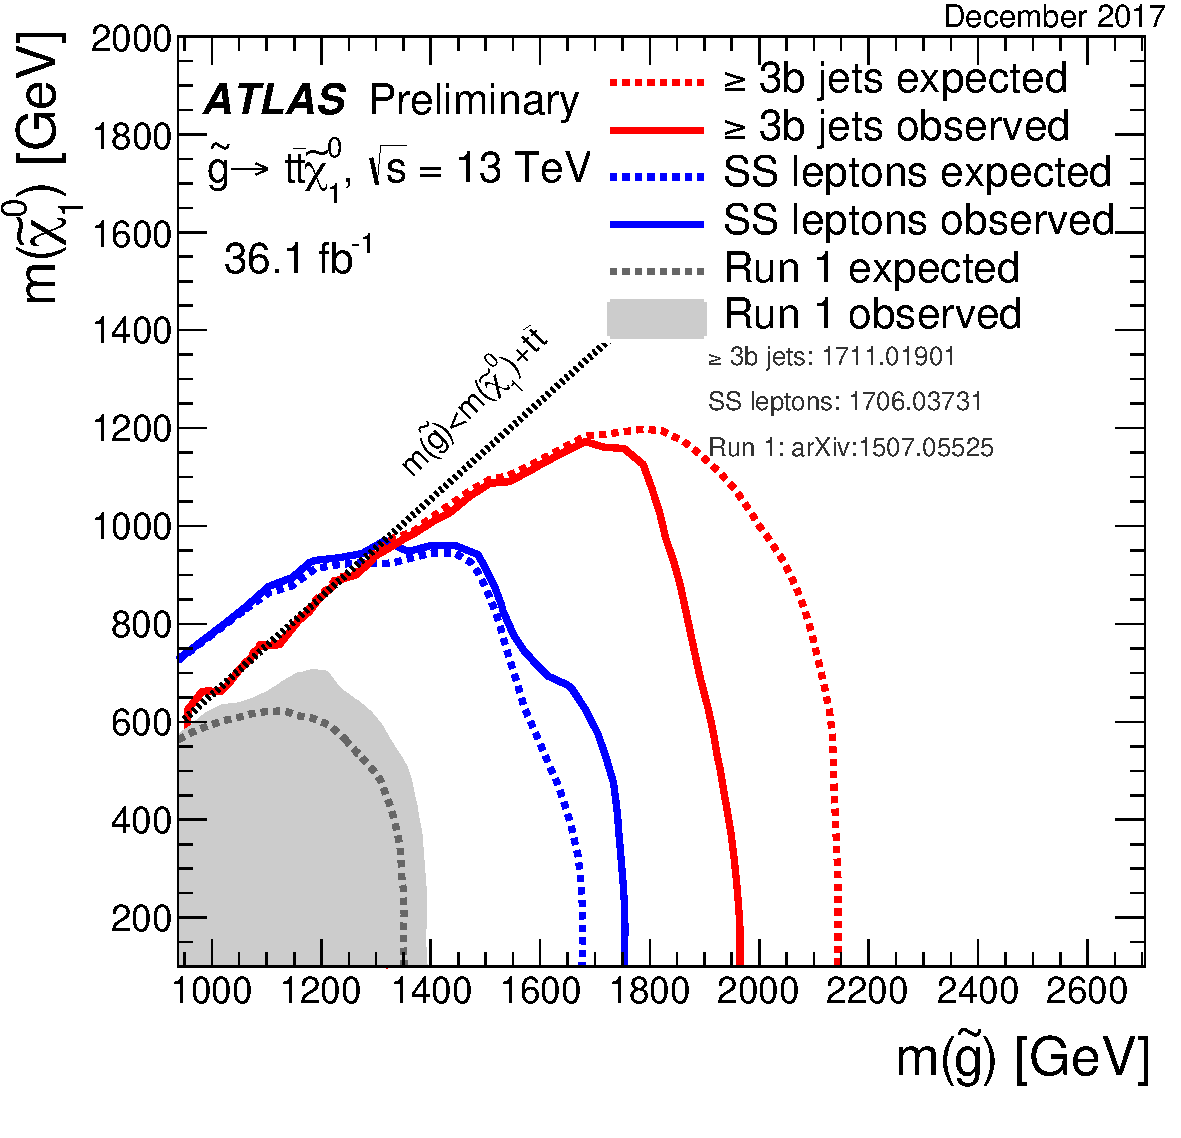
\includegraphics[width=0.65\textwidth]{./fig/limits/ATLAS_SUSY_Gtt.pdf}
\end{center}
\caption[ATLAS Gluino-mediated stop production limits]{ATLAS Gluino-mediated stop production limits in the $(m_{\tilde{g}}, m_{\tilde{chi}_1^0})$ plane.}
\label{fig:ATLASgluinolimits}
\end{figure}

\subsubsection{Direct stop pair production}

Figure \ref{fig:ATLASstoplimits} shows a summary of the dedicated ATLAS searches for top squark (stop) pair production based on 20 \ifb of p-p collision data taken at \cmotto TeV, and 4.7 \ifb of p-p collision data taken at \cmotto TeV \cite{atlas:stop0lep} \cite{atlas:stop2lep}. Exclusion limits at 95\% CL are shown in the $\left( m_{\tilde{t}_1}, m_{\tilde{\chi}^+_1} \right)$ plane. The dashed and solid lines show the expected and observed limits, respectively, including all uncertainties except the theoretical signal cross-section uncertainty. Three decay modes are considered separately with 100\% BR: 

\begin{itemize}
\item $\tilde{t} \rightarrow t \tilde{\chi}^0_1$ (7 TeV: \cite{atlas:stoplim_1} \cite{atlas:stoplim_2} \cite{atlas:stoplim_3}, 8 TeV \cite{atlas:stoplim_4} \cite{atlas:stoplim_5} \cite{atlas:stoplim_6}, where the $\tilde{t}_1$ is mostly right-handed)


\item $\tilde{t} \rightarrow W b  \tilde{\chi}^0_1$ (3-body decay for $m_{\tilde{t}} < m_t + m_{\tilde{\chi}^0_1} $, 8 TeV \cite{atlas:stoplim_4}\cite{atlas:stoplim_6}) 

\item  $\tilde{t} \rightarrow f f' b  \tilde{\chi}^0_1$ (4-body decay, 8 TeV \cite{atlas:stoplim_4}\cite{atlas:stoplim_7}). The region stop1 mass below 100 GeV has not been considered in \cite{atlas:stoplim_4} for the 4-body decay. 

\end{itemize}

\begin{figure}[htbp]
\begin{center}
%\includegraphics[width=0.65\textwidth]{./fig/limits/ATLAS_SUSY_Stop_tLSP.pdf}
\end{center}
\caption[ATLAS limits on direct stop production]{ATLAS limits on direct stop production in the $\left( m_{\tilde{t}_1}, m_{\tilde{\chi}^+_1} \right)$ plane.}
\label{fig:ATLASstoplimits}
\end{figure}



\subsubsection{Electroweak chargino-neutralino production}

Figure \ref{fig:ATLASewlimits} shows the summary of ATLAS searches for electroweak production of charginos and neutralinos based on 20 \ifb of p-p collision data at \cmotto TeV. Exclusion limits at 95\% confidence level are shown in the $\left( m_{\tilde{\chi}^+_1}, m_{\tilde{\chi}^0_1}  \right)$ plane. The dashed and solid lines show the expected and observed limits, respectively, including all uncertainties except the theoretical signal cross-section uncertainties. Four decay modes of the charginos and neutralinos are considered separately with 100\% branching fraction: 

\begin{itemize}

\item $\tilde{\chi}^+_1 \rightarrow \tilde{l} \nu (\tilde{\nu} l ) \rightarrow l \nu \tilde{\chi}^0_1 $, $\tilde{\chi}^0_2  \rightarrow \tilde{l} l (\tilde{\nu} \nu ) \rightarrow l l \tilde{\chi}^0_1 ( \nu \nu \tilde{\chi}^0_1  )$, resulting in BR(3 leptons)=50\% and BR(2 leptons)=100\% for $\tilde{\chi}^+_1 + \tilde{\chi}^0_2$ and $\tilde{\chi}^+_1 + \tilde{\chi}^+_1$ productions, respectively. The decays via sleptons and sneutrinos occur with 50\% probability each. 

\item $\tilde{\chi}^+_1 \rightarrow \tilde{\tau} \nu_{\tau} \tilde{\nu} \rightarrow \tau \nu \tilde{\chi}^0_1$,  $\tilde{\chi}^0_2  \rightarrow \tilde{\tau} \tau ( \tilde{\nu} \nu ) \rightarrow \tau \tau \tilde{\chi}^0_1 ( \nu \nu \tilde{\chi}^0_1   ) $, resulting in BR(3 taus)=50\% and BR(2 taus)=100\% for $\tilde{\chi}^+_1 + \tilde{\chi}^0_2$ and $\tilde{\chi}^+_1 + \tilde{\chi}^+_1$ productions respectively. The decays via staus and tau sneutrinos occur with 50\% probability each. 

\item $\tilde{\chi}^+_1 \rightarrow W  \tilde{\chi}^0_1$, $\tilde{\chi}^0_2  \rightarrow Z \tilde{\chi}^0_1$.

\item $\tilde{\chi}^+_1 \rightarrow W  \tilde{\chi}^0_1$, $\tilde{\chi}^0_2  \rightarrow H \tilde{\chi}^0_1$, where H is the Higgs boson and decays with the SM branching ratios.

\end{itemize}

\begin{figure}[htbp]
\begin{center}
%\includegraphics[width=0.65\textwidth]{./fig/limits/ATLAS_SUSY_EWSummary.pdf}
\end{center}
\caption[ATLAS Electroweak chargino-neutralino production limits]{ATLAS limits for Electroweak chargino-neutralino production in the $\left( m_{\tilde{\chi}^+_1}, m_{\tilde{\chi}^0_1}  \right)$ plane.}
\label{fig:ATLASewlimits}
\end{figure}

\begin{figure}[p]
\begin{center}
%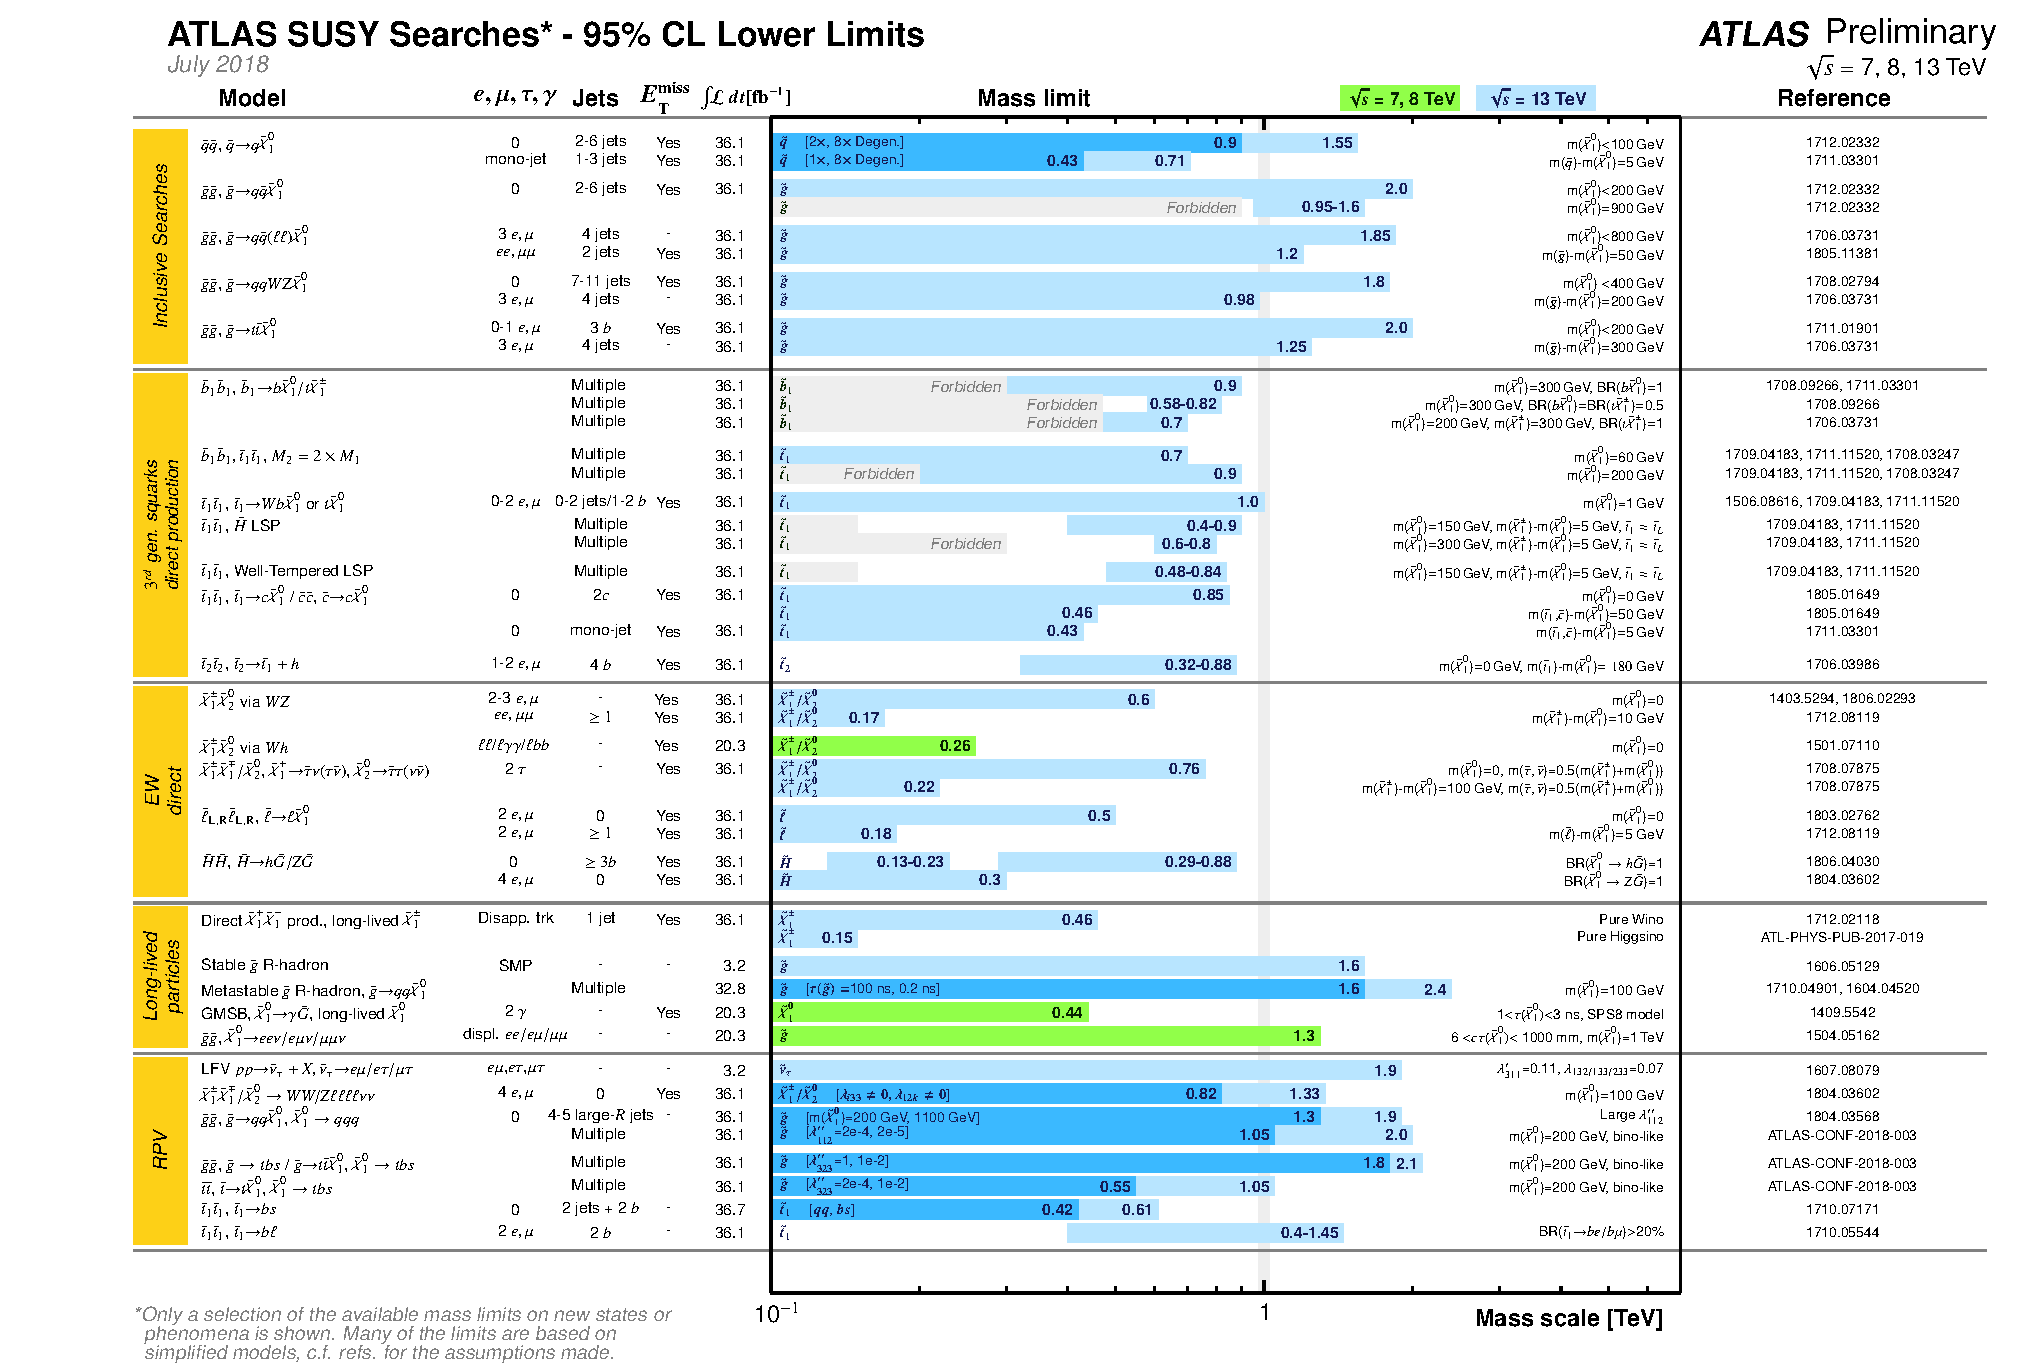
\includegraphics[width=\textwidth]{./fig/limits/ATLAS_SUSY_Summary.pdf}
\end{center}
\caption[Mass reach of ATLAS searches for Supersymmetry]{Mass reach of ATLAS searches for Supersymmetry.}
\label{fig:SUSYlimits}
\end{figure}


%%%%%%%%%%%%%%%%%%%%%%%%%%%%%%%%%%%%%%%%%%
%%%%%%%%%%%%%%%%%%%%%%%%%%%%%%%%%%%%%%%%%%






